\documentclass[zavrsnirad]{fer}
% Dodaj opciju upload za generiranje konačne verzije koja se učitava na FERWeb
% Add the option upload to generate the final version which is uploaded to FERWeb


\usepackage{blindtext}
\usepackage{mathrsfs}
\usepackage{float}
\usepackage[shortlabels]{enumitem}
\usepackage{mathtools}
\usepackage{microtype}
\usepackage{hyperref}
\usepackage{listings}
\usepackage{xcolor}
\usepackage{caption}
\usepackage{chngcntr}


\lstset{
  language=C++,
  basicstyle=\ttfamily\small,
  keywordstyle=\color{blue},
  commentstyle=\color{gray},
  stringstyle=\color{orange},
  numbers=left,
  numberstyle=\tiny,
  stepnumber=1,
  numbersep=10pt,
  tabsize=2,
  showspaces=false,
  showstringspaces=false,
  breaklines=true,
  breakatwhitespace=true,
  frame=single,
}

\newtheorem{definition}{Definicija}
\renewcommand{\thedefinition}{\arabic{definition}.}

\newtheorem{theorem}{Teorem}
\renewcommand{\thetheorem}{\arabic{theorem}.}

\newtheorem{proof}{Dokaz}
\renewcommand{\theproof}{\arabic{proof}.}

\newtheorem{algorithm}{Algoritam}
\renewcommand{\thealgorithm}{\arabic{algorithm}.}


\newenvironment{proof*}
{\begin{proof}\renewcommand{\theproof}{}}
  {\end{proof}}





%--- PODACI O RADU / THESIS INFORMATION ----------------------------------------

% Naslov na engleskom jeziku / Title in English
\title{Development of an application for risk assessment in investment
portfolios with the help of Monte Carlo simulations}

% Naslov na hrvatskom jeziku / Title in Croatian
\naslov{Razvoj aplikacije za procjenu rizika
u investicijskim portfeljima uz pomoć Monte Carlo simulacija}

% Broj rada / Thesis number
\brojrada{1951}

% Autor / Author
\author{Ivan Džanija}

% Mentor
\mentor{Prof.\@ Mihaela Vranić}

% Datum rada na engleskom jeziku / Date in English
\date{June, 2025}

% Datum rada na hrvatskom jeziku / Date in Croatian
\datum{lipanj, 2025.}

%-------------------------------------------------------------------------------


\begin{document}
\renewcommand{\lstlistingname}{Kod}
\renewcommand{\thelstlisting}{\thesection\arabic{lstlisting}}

% Naslovnica se automatski generira / Titlepage is automatically generated
\maketitle

%--- ZADATAK / THESIS ASSIGNMENT -----------------------------------------------

% Zadatak se ubacuje iz vanjske datoteke / Thesis assignment is included from external file
% Upiši ime PDF datoteke preuzete s FERWeb-a / Enter the filename of the PDF downloaded from FERWeb
\zadatak{zadatak.pdf}

%--- ZAHVALE / ACKNOWLEDGMENT --------------------------------------------------

\begin{zahvale}
	% Ovdje upišite zahvale / Write in the acknowledgment
	Hvala na svemu puno.
	ovo je test i opet
\end{zahvale}

% Odovud započinje numeriranje stranica / Page numbering starts from here
\mainmatter

% Sadržaj se automatski generira / Table of contents is automatically generated
\tableofcontents

%--- UVOD / INTRODUCTION -------------------------------------------------------
\chapter{Uvod}
\label{pog:uvod}

Modeliranje ponašanja portfelja je jedna od ključnih metoda pri odabiru
investicijskog pristupa. Od odabira pojedinačnih dionica, raznih
derivata, sigurnih obveznica ili investicijkih fondova sve do mogućnosti
čuvanja novčanih rezervi.\\
U posljednjem desetljeću, kriptovalute su postale sveprisutna
komponenta financijskih tržišta, karakterizirana visokom volatilnošću,
nelinearnim ovisnostima i globalnom dostupnošću što kroz iznimno pouzdane izvore
što kroz izrazito nepouzdane izvore.
Upravljanje rizikom u takvom okruženju zahtijeva napredne alate za
modeliranje budućih scenarija.
Jedan od takvih alata u standarnim financijskim modelima je Monte Carlo
simulacija.\\
Monte Carlo simulacija, kao statistička metoda temeljena na ponovljenom
uzorkovanju slučajnih varijabli i često korištena metoda u modeliranju
ostalih financijskih instrumenata, nameće se kao potencijalno uspješan
pristup za analizu portfelja kriptovaluta.\\
U ovom radu fokusira se na ručnoj implementaciji svih matematičkih
operacija i modela u \texttt{C++} programskom jeziku bez korištenja
vanjskih biblioteka potrebnih za modeliranje i provođenje Monte
Carlo simulacija. Cilj je stečeno znanje na kolegijima primjeniti
na barem naivne implementacije kako bi se moglo usporediti rad takog
pristupa sa razvijenim i maksimalno optimiziranim bibliotekama.\\
To uključuje Monte Carlo metodu za predviđanje vrijednosti portfelja s primjenom
Cholesky dekompozicije kako bi se osigurala realistična obrada
korelacija između kriptovaluta koje su još uvijek specijalna skupina investicija
s visokom međusobnom korelecijom.\\
Osim Monte Carlo simulacija za predviđanje budućih cijena portfelja,
implementira se i PCA (Principal Component Analysis) dekompozicija
kao jedna od jednostavnih metoda za efikasnu diverzifikaciju portfelja
i samim time smanjenje rizika upravo kroz smanjenje dimenzionalnosti podataka
i identifikaciju glavnih komponenti koje objašnjavaju najveći dio
varijance podataka.\\
Glavni izazov u modeliranju kriptovaluta leži u njihovoj inherentnoj
nestabilnosti. Dok tradicionalne financijske instrumente karakteriziraju
relativno predvidljivi obrasci, kriptovalute pokazuju ekstremne fluktuacije
koje zahtijevaju precizno podešavanje parametara poput driftova i
volatilnosti. Osim velike i teško predvidive volatilnosti dodatan problem
predstavlja kratak period postojanja tog financijskog instrumenta.
Većina kriptovaluta postoji tek nekoliko godina, a neke su čak i
nestale samo nekoliko mjeseci nakon što su se pojavile. Period manji od
10 godina je u financijskom svijetu vrlo kratak pogotovo ako uzmemo u obzir
da nije bilo prevelikih promjena ili kriza na financijskim tržištima
u vremenu postojanja kriptovaluta.\\
U radu je razvijen \texttt{C++} programski okvir koji integrira povijesne podatke
kriptovaluta, obavlja potrebne matematičke operacije i generira simulacije.
Generirane simulacije omogućuju analizu različitih scenarija kretanja cijena,
a korisnik može odabrati različite portfelje i vremenske okvire.
Sva interakcija s korisnikom odvija se putem grafičkog sučelja koje
omogućuje jednostavno upravljanje parametrima simulacije i vizualizaciju
rezultata.\\
Rad je strukturiran kako slijedi: U drugom poglavlju opisuju se teorijske
osnove teorije portfelja, Monte Carlo metode, PCA dekompozicija te
sve potrebne matematičke osnove i teorije potrebne za razumijevanje
i implementaciju modela.
Treće poglavlje detaljno opisuje implementaciju algoritama i struktura, uključujući
model portfelja, model kriptovalute, postupke poput Cholesky dekompozicije,
traženja svojstvene dekompozicije, brzog ``parsiranja`` financijskog skupa podataka
i optimizacije za velike skupove podataka.
U četvrtom poglavlju analiziraju se rezultati simulacija za različite
konfiguracije portfelja, dok se u zaključku raspravlja o primjenjivosti
modela, mogućim i očitim praktičnim problemima i smjerovima daljnjeg istraživanja.

Ovakav rad može poslužiti kao osnova za daljnje istraživanje i razvoj
naprednijih modela i aplikacija koji će omogućiti bolje razumijevanje i upravljanje
rizicima povezanima s kriptovalutama, ali i ostalim financijskim instrumentima.
Pogotovo jer se kroz izradu sustava i aplikacije kao sekundarni rezultat
pokrenuo razvitak biblioteke za rad s financijskim podatcima i potrebnim
matematičkim okvirima koja će se moći koristiti u budućim radovima i projektima.

%-------------------------------------------------------------------------------
\chapter{Teorija portfelja i matematičke osnove}
\label{pog:teorija_portelja}
Teorija portfelja, čiji su začetnici Harry Markowitz i James Tobin,
daje strogu matematičku definiciju financijskim pojmovima.
Ključni optimizacijski problem teorije portfelja je
\textit{dualni cilj}: maksimizacija očekivanog povrata
uz istovremeno minimiziranje rizika.

\section{Investicije}
\label{sek:investicije}
Investicija ili ulaganje je proces alokacije ograničenih resursa
kao što su novac, vrijeme ili energija u svrhu ostvarivanja
većeg povrata ili dodatne koristi u budućnosti \cite{Investments}.
Ovime kažemo kako investicija ne mora nužno biti financijska,
ali u ovom radu se fokusiramo na financijske investicije koje nam
predstavljaju izdvajanje i ulaganje novca u različite financijske instrumente
kroz određeni vremenski period s ciljem ostvarivanja većeg povrata
u budućnosti ili smanjenje gubitka vrijednosti novca.

\section{Portfelj}
\label{sek:portfelj}
Investicijske portfelje matematički prikazujemo kao linearnu kombinaciju
pojedinih investicija sa vektorom pojedinih udjela $\mathbf{w}$.
\begin{definition}
	Vektor $\mathbf{w}$ predstavlja udjele investicija u portfelju.
\end{definition}
\begin{align*}
	\mathbf{w} = \begin{pmatrix} w_1 \\ w_2 \\ \dots \\ w_N \end{pmatrix},
	\indent \sum_{i = 1}^{N} w_i = 1
\end{align*}

\section{Povrati}
\label{sek:povrati}
Povrat investicije je osnovna mjera uspješnosti investicije.
\subsection{Aritmetički povrat}

\begin{definition}
	Neka je $P_t$ cijena financijskog instrumenta u trenutku $t$ te
    $P_{t-1}$ cijena istog instrumenta u trenutku $t-1$. Aritmetički povrat
    $R_t$ definiramo kao:
\end{definition}
\begin{align*}R_t = \frac{P_t}{P_{t-1}} - 1 =
    \frac{P_t - P_{t-1}}{P_{t-1}} =
\frac{\Delta P}{P_{t-1}}
\end{align*}

\noindent Neka buduća cijena nam neće biti poznata pri investiranju te
zato povrat promatramo kao slučajnu varijablu.
Vidimo kako je moguće imati negativan povrat ako je cijena koju
promatramo manja od početne cijene i to je upravo situacija koji
pokušavamo izbjeći.

\subsection{Logaritamski povrat}
Logaritamski povrat $r_t$ definiramo preko prirodnog logaritma omjera cijena.

\begin{definition}
    Neka je $P_t$ cijena financijskog instrumenta u trenutku $t$ te
    $P_{t-1}$ cijena istog instrumenta u trenutku $t-1$. Logaritamski povrat
    $r_t$ definiramo kao:
\end{definition}
\begin{align*}
    r_t = \ln\left(\frac{P_t}{P_{t-1}}\right) = \ln(P_t) - \ln(P_{t-1})
\end{align*}
\noindent Logaritamski povrat u pravilu koristimo zbog njegovih pogodnih
matematičkih svojstava kao što je svojstvo simetrije $\ln(a) = -\ln(1/a)$
te svojstvo aditivnosti $r_{0,T} = \sum_{t=1}^T r_t$.

\subsection{Očekivani povrat }
\label{sek:ocekivani_povrat}
\begin{definition}
	Očekivani povrat promatramo kao srednju vrijednost prijašnjih
	povrata jer je upravo srednja vrijednost nepristran procjenitelj
	očekivanja slučajne varijable $R_t$ za koji vrijedi:
\end{definition}
\begin{align*}
	E(R_t) =\frac{1}{N} \sum_{i = 1}^{N} R_i
\end{align*}
\begin{definition}
Očekivani povrat portfelja je linearna kombinacija očekivanih povrata pojedinačnih asseta:
\end{definition}
\begin{align*}
\mathbb{E}[R_p] =
    \mathbf{w}^\intercal \boldsymbol{\mu} = \sum_{i=1}^n w_i \mu_i
\end{align*}
\indent gdje je $\boldsymbol{\mu} = (\mu_1, \dots, \mu_n)^\intercal$ vektor očekivanih povrata.

\section{Volatilnost}
Drugi dio optimizacijskog problema teorije portfelja je smanjenje rizika.
Volatilnost je upravo jednostavna mjera rizika koja ima pogodna matematička svojstva.
Promatramo je kao standardnu devijaciju slučajne varijable $R_t$, a ima je smisla tako promatrati
jer će nam upravo takva mjera kvantificirati kretanje povrata.
\begin{definition}
	Volatilnost investicije definiramo kao nepristran procjenitelj
	standardne devijacije slučajne varijable $R_t$:
\end{definition}
\begin{align*}
	\sigma_R = \sqrt{\frac{1}{N - 1} \sum_{i = 1}^{N} \left[R_i - E(R_t)\right]^2}
\end{align*}
\begin{definition}
Volatilnost portfelja mjeri se standardnom devijacijom povrata i dana je kvadratnim korijenom varijance:
\end{definition}
\begin{align*}
\sigma_p = \sqrt{\mathbf{w}^\intercal \boldsymbol{\Sigma} \mathbf{w}}
\end{align*}
\indent gdje je $\boldsymbol{\Sigma}$ matrica kovarijance s elementima $\Sigma_{ij} = \text{Cov}(r_i, r_j)$.

\section{Geometrijsko Brownovo gibanje}
\label{sek:gbm}
Geometrijsko Brownovo gibanje (GBM) je jedan od standardnih
stohastičkih procesa za modeliranje kretanja cijena financijskih instrumenata.
Diferencijalna jednadžba GBM-a je:
\begin{align*}
    dS_t = \mu S_t dt + \sigma S_t dW\left(t\right)
\end{align*}
\indent gdje je $W\left(t\right)$ Wienerov proces.\\
Eksplicitno rješenje GBM-a daje formulu za cijenu u trenutku $t$:

\begin{align*}
S_t = S_0 \exp\left[\left(\mu - \frac{\sigma^2}{2}\right)t +
    \sigma W_t\right]
\end{align*}
\indent gdje je $S_0$ početna cijena, $\mu$ drift, $\sigma$ volatilnost i $W_t$
Wienerov proces.\\
Detaljno objašnjene GBM-a i njegovih svojstava te kompletan derivacijski
postupak možete pronaći u \cite{GMBIzvod}.

\section{Monte Carlo simulacije}
\label{sek:monte_carlo}
Monte Carlo metoda je numerička metoda koja koristi slučajno
uzorkovanje za rješavanje problema.
Jedan iznimno intuitivan i elegantan primjer je određivanje
vrijednost broja $\pi$.
Ideja je generiranje što većeg broja točaka unutar jediničnog
kvadrata koji u sebi sadrži jedinični krug te određivanje
omjera broja točaka unutar kruga i ukupnog broja točaka te onda
preko omjera površina kvadrata i kruga dobijemo procjenu vrijednosti
broja $\pi$.

U kontekstu financija, Monte Carlo simulacije koriste se za
generiranje vjerojatnosnih scenarija budućih cijena.
Za portfelj od $n$ instrumenata, koraci su:
\begin{enumerate}
    \item Generiraj nezavisne slučajne varijable $Z_i \sim N(0,1)$ (i.i.d.)
\item Transformiraj slučajni vektor nezavisnih varijabli $Z$ u
    slučajni vektor koreliranih varijabli $\mathbf{Y} = L\mathbf{Z}$
    gdje je $L$ donje trokutasta matrica Cholesky
        dekompozicije $\boldsymbol{\Sigma}$
\item Ažuriraj cijene simulacije po GBM formuli za svaki instrument:
\begin{align*}
S_t^{(i)} = S_0^{(i)} \exp\left(\left(\mu_i - \frac{\sigma_i^2}{2}\right)\Delta t + \sigma_i Y_i \sqrt{\Delta t}\right)
\end{align*}
\item Izračunaj vrijednost portfelja $V_t = \sum_{i=1}^n w_i S_t^{(i)}$
\end{enumerate}

\section{Cholesky dekompozicija}
\label{sek:cholesky}
Cholesky dekompozicija je numerička metoda koja se koristi za
dekompoziciju simetričnih pozitivno definitnih matrica. I upravo
je matrica kovarijance $\boldsymbol{\Sigma}$ simetrična pozitivno
definitna matrica. Teorem u \cite{NumerickaMatematika}.
\begin{definition}
    \label{def:cholesky}
    Neka je $\boldsymbol{\Sigma}$ simetrična pozitivno definitna
    matrica kovarijance. Tada postoji jedinstvena donja trokutasta
    matrica $L$ takva da:
    \begin{align*}
        \boldsymbol{\Sigma} = LL^\intercal
    \end{align*}
    \indent gdje je $L$ donja trokutasta matrica.
\end{definition}
Ova faktorizacija omogućuje generiranje vektora koreliranih slučajnih varijabli
iz vektora nezavisnih slučajnih varijabli.

\begin{theorem}
Neka je $\mathbf{Z} = (Z_1, ..., Z_n)^\intercal$ vektor nezavisnih $N(0,1)$ varijabli. Tada vektor $\mathbf{Y} = L\mathbf{Z}$ ima kovarijacijsku matricu $\boldsymbol{\Sigma}$.
\end{theorem}
\begin{proof}
\begin{align*}
\text{Cov}(\mathbf{Y}) = \mathbb{E}[L\mathbf{Z}(L\mathbf{Z})^\intercal] -
    \mathbb{E}[L\mathbf{Z}]\mathbb{E}[(L\mathbf{Z})^\intercal]
    = L\mathbb{E}[\mathbf{Z}\mathbf{Z}^\intercal]L^\intercal - 0
    = L \cdot I \cdot L^\intercal = LL^\intercal = \boldsymbol{\Sigma}
\end{align*}
\end{proof}

\section{PCA dekompozicija}
\label{sek:pca}
PCA (Principal Component Analysis) je tehnika koja se koristi za
redukciju dimenzionalnosti podataka i identifikaciju glavnih komponenti koje
objašnjavaju što veći dio ukupne varijance podataka. Ovo nam omogućuje
najefikasniju diverzifikaciju portfelja i samim time smanjenje
rizika \cite{Investments}.

\begin{definition}
    Neka je $\boldsymbol{\Sigma}$ kovarijacijska matrica slučajnog
    vektora $\mathbf{X} = (X_1, X_2, \dots, X_n)^\intercal$.
    Svojstvena dekompozicija matrice
    $\boldsymbol{\Sigma}$ daje:
\end{definition}
\begin{align*}
    \boldsymbol{\Sigma} = \boldsymbol{V} \boldsymbol{\Lambda} \boldsymbol{V}^\intercal
\end{align*}
\indent gdje je $\boldsymbol{V}$ ortogonalna matrica vlastitih vektora, a
$\boldsymbol{\Lambda}$
dijagonalna matrica vlastitih vrijednosti.\\

\noindent Ovaj rezultat sljedi iz spektralnog teorema \cite{NumerickaLinearna}.
Sada možemo definirati PCA dekompoziciju.
\begin{definition}
    PCA dekompozicija slučajnog vektora $\mathbf{X}$ daje novi vektor
    $\mathbf{Y} = (Y_1, Y_2, \dots, Y_n)^\intercal$ gdje su $Y_i$
    glavne komponente slučajnog vektora $\mathbf{X}$.\\
    Glavne komponente su linearne kombinacije originalnih varijabli
    $\mathbf{X}$ i definiraju se kao:
    \begin{align*}
        \mathbf{Y} = \boldsymbol{V}^\intercal \mathbf{X}
    \end{align*}
    \indent gdje je $\boldsymbol{V}$ matrica vlastitih vektora kovarijacijske
    matrice $\boldsymbol{\Sigma}$, a $Y_i$ su glavne komponente.
\end{definition}




%--- IMPLEMENTACIJA / IMPLEMENTATION -------------------------------------------
\chapter{Implementacija aplikacije}
\label{pog:implementacija}
Ovaj dio rada opisuje implementaciju aplikacije za simulaciju
portfelja kriptovaluta. Aplikacija je napisana u \texttt{C++} programskom
jeziku i koristi isključivo standardnu biblioteku \texttt{C++} za matematičke
operacije i modeliranje. Za interakciju s korisnikom koristi se
grafičko sučelje(implementirano sa Qt bibliotekom za \texttt{C++}) koje
omogućuje vizualizaciju rezultata. Prikaz modela rada aplikacije
je dan na slici \ref{fig:model_aplikacije}.
\\

\begin{figure}[H]
    \centering
    \includegraphics[width=1.0\textwidth]{Figures/model_aplikacije.png}
    \caption{Model rada aplikacije}
    \label{fig:model_aplikacije}
\end{figure}

\section{Podatci}
\label{sek:podaci}
Podatci korišteni u aplikaciji su povijesne vrijednosti
kriptovaluta preuzete sa stranice \cite{kaggledataset}.
Podatci su u CSV formatu i sadrže informacije o otvorenoj, zatvorenoj,
najvišoj i najnižoj cijeni te volumenu kriptovalute i ukupnom tržišnom
kapitalu za svaki vremenski interval. Za potrebe aplikacije,
ovaka pristup je dovoljan jer se fokusiramo na analizu i
implementaciju modela portfelja i potrebnih matematičkih operacija.
U budućnosti bi se mogla implementirati i dohvaćanje podataka
u realnom vremenu preko nekog javno dostupnog API-ja. Time bi
aplikacija postala korisna i za praćenje portfelja u realnom vremenu.\\
U trenutnim podatcima nalaze se povijesne vrijednosti za 23 različite kriptovalute.
\begin{itemize}
    \item Aave (AAVE)
    \item Bitcoin (BTC)
    \item Ethereum (ETH)
    \item Binance Coin (BNB)
    \item Crypto.com Coin (CRO)
    \item Cardano (ADA)
    \item Solana (SOL)
    \item Ripple (XRP)
    \item Polkadot (DOT)
    \item Dogecoin (DOGE)
    \item Litecoin (LTC)
    \item Chainlink (LINK)
    \item Uniswap (UNI)
    \item Bitcoin Wrapped (WBTC)
    \item Stellar (XLM)
    \item TRON (TRX)
    \item Cosmos (ATOM)
    \item Monero (XMR)
    \item Thether (USDT)
    \item USD Coin (USDC)
    \item Eos (EOS)
    \item Iota (IOTA)
    \item NEM (XEM)
\end{itemize}


%--- ALGORITMI / ALGORITHMS ----------------------------------------------------
\section{Algoritmi i komponente}
\label{sek:algoritmi_i_komponente}
Aplikacija se sastoji od nekoliko ključnih komponenti:
\begin{itemize}
    \item \textbf{Parsiranje podataka (\ref{sek:parsiranje_podataka}):} učitavanje i obrada povijesnih
    podataka o cijenama kriptovaluta.

\item \textbf{Model kriptovaluta (\ref{sek:model_kriptovalute}):} Implementacija modela kriptovaluta.

    \item \textbf{Model portfelja (\ref{sek:model_portfelja}):} Definiranje portfelja kriptovaluta.

    \item \textbf{Matematički okvir (\ref{sek:matematicki_okvir}):} Implementacija matematičkih
    operacija potrebnih za simulaciju i modeliranje portfelja. Npr.
        (Množenje matrica, vektora, operacije nad vektorima i matricama te
        razne matrične dekompozicije).

    \item \textbf{Monte Carlo simulacija (\ref{sek:monte_carlo_simulacija}):} Generiranje simulacija
    budućih cijena portfelja kriptovaluta.

    \item \textbf{PCA dekompozicija (\ref{sek:pca_dekompozicija}):} Implementacija PCA dekompozicije
    za redukciju dimenzionalnosti podataka i identifikaciju glavnih
    komponenti.

    \item \textbf{Vizualizacija rezultata (\ref{sek:vizualizacija_rezultata}):} Prikaz rezultata simulacija
    kroz grafičko sučelje.
\end{itemize}


\subsection{Parsiranje podataka}
\label{sek:parsiranje_podataka}
Efikasno parsiranje povijesnih podataka o cijenama kriptovaluta
je prvi korak u simulaciji i stavaranju modela portfelja.
Podatci se učitavaju iz CSV datoteka koje sadrže povijesne cijene
kriptovaluta. Povijesni podatci su preuzeti sa \cite{kaggledataset}.
Podatci se parsiraju u \emph{candle} strukturu koja sadrži
otvorenu, zatvorenu, najvišu i najnižu cijenu te volumen
kriptovalute za svaki vremenski interval. Također se pri parsiranju
računaju i logaritamski povrati za svaki vremenski interval te se izvršava
poravnanje vremenskih oznaka svih kriptovaluta. U pravilu se kriptovaluta može
i trguje 24/7, ali je problem bio što neke kriptovalute nisu postojale ili
nisu imale podatke za sve dane svih ostalih kriptovaluta.
\begin{lstlisting}[caption={Struktura \emph{candle} koja sadrži povijesne
podatke o cijenama kriptovaluta}, label={lst:candle}]
struct Candle {
  public:
    // OHLC
    double open, high, low, close;
    double volume, marketcap;
    timestamp time;
    double log_return;

    // Constructors, getters, setters, etc.
};
\end{lstlisting}

\subsection{Model kriptovalute}
\label{sek:model_kriptovalute}
Model kriptovalute je implementiran kao klasa koja
sadrži povijesne podatke o cijenama kriptovalute
i metode za izračunavanje povrata, volatilnosti
i driftova.
\begin{lstlisting}[caption={Model kriptovalute}, label={lst:kriptovaluta}]
class Cryptocurrency {
  public:
    std::string name, tick;
    std::vector<Candle> hist_data;
    bool metrics_calculated = false;

    // Drift = sum(return_i) / n;
    // Volatility = sqrt((1/n - 1) * sum((return_i - Drift)^2)
    double drift, volatility;

    // Constructors, getters, setters, etc.

    void calculate_metrics();
    void reevaluate_metrics();
    void individual_monte_carlo(int sim_count, int forecast_days);
};
\end{lstlisting}

\subsection{Model portfelja}
\label{sek:model_portfelja}
Model portfelja je implementiran kao klasa koja
sadrži vektor kriptovaluta i njihove udjele u portfelju.
\begin{lstlisting}[caption={Model portfelja}, label={lst:portfelj}]
class Portfolio {
  private:
    std::vector<std::string> _asset_names;
    std::unordered_map<Cryptocurrency, double, Cryptocurrency::Hash> _assets;

  public:
    // Covariance matrix
    Doubles_Matrix aligned_log_return_matrix;
    Doubles_Matrix covariance_matrix;
    std::vector<double> aligned_means;
    std::vector<double> aligned_volatilities;

    timestamp aligned_start = timestamp();
    timestamp aligned_end = timestamp();
    timestamp aligned_stamp = timestamp();
    bool aligned_returns_calculated = false;
    bool covariance_matrix_calculated = false;
    bool aligned_metrics_calculated = false;

    void add_asset(const Cryptocurrency &crypto, double ammount);

    void remove_asset(const Cryptocurrency &crypto, double ammount);

    Cryptocurrency get_asset(const std::string &name) const;

    std::vector<std::string> &get_asset_names();

    Doubles_Matrix &aligned_log_returns(timestamp start);
    Doubles_Matrix &calculate_covariance(timestamp start);
    int calculate_aligned_metrics(timestamp start);
    std::vector<Doubles_Matrix> monte_carlo(int simulations, int steps,
                                            timestamp start);
    int PCA(timestamp start, int num_components,
            std::vector<std::pair<double, std::vector<double>>> &components,
            double &total_variance, double &variance_explained);
};
\end{lstlisting}

\subsection{Matematički okvir}
\label{sek:matematicki_okvir}
Matematički okvir aplikacije implementira osnovne matematičke
operacije nad vektorima i matricama, kao što su množenje
matrica i vektora te razne matrične dekompozicije. Sve metode koriste
samo standardnu biblioteku \texttt{C++}.

\begin{lstlisting}[caption={Metode implementirane u matematičkom okviru}, label={lst:cpp_example}]
template <typename T>
std::vector<std::vector<T>>
matrix_transpose(const std::vector<std::vector<T>> &matrix);

template <typename T>
int cholesky_decomposition(const std::vector<std::vector<T>> &matrix,
                           std::vector<std::vector<T>> &L);
template <typename T> double vector_norm(const std::vector<T> &v);

template <typename T> std::vector<T> normalized(const std::vector<T> &v);

template <typename T>
std::vector<T> scalar_multiply(const std::vector<T> &v, T scalar);

template <typename T>
std::vector<std::vector<T>>
matrix_scalar_multiply(const std::vector<std::vector<T>> &matrix, T scalar);

template <typename T>
std::vector<T> vector_add(const std::vector<T> &v1, const std::vector<T> &v2);

template <typename T>
std::vector<T> vector_subtract(const std::vector<T> &v1,
                               const std::vector<T> &v2);

template <typename T>
std::vector<T> vector_multiply(const std::vector<T> &v1,
                               const std::vector<T> &v2);

template <typename T>
std::vector<std::vector<T>>
matrix_multiply(const std::vector<std::vector<T>> &A,
                const std::vector<std::vector<T>> &B);

template <typename T>
std::vector<std::vector<T>>
matrix_subtract(const std::vector<std::vector<T>> &A,
                const std::vector<std::vector<T>> &B);



template <typename T>
int QR_decomposition(const std::vector<std::vector<T>> &matrix,
                     std::vector<std::vector<T>> &Q,
                     std::vector<std::vector<T>> &R);

template <typename T> int normalize(std::vector<T> &v);

template <typename T>
int matrix_inverse(const std::vector<std::vector<T>> &input,
                   std::vector<std::vector<T>> &output) {

template <typename T>
std::vector<T> eigen_values(const std::vector<std::vector<T>> &matrix);

template <typename T>
int eigen_pairs(const std::vector<std::vector<T>> &matrix,
                std::vector<std::pair<T, std::vector<T>>> &results);
\end{lstlisting}

\subsubsection{Cholesky dekompozicija}
\label{sek:cholesky_dekompozicija}
Cholesky dekompozicija je implementirana
kao metoda koja prima kovarijacijsku matricu i matricu $L$ u koju se sprema
donja trokutasta matrica dekompozicije te metoda vraća \texttt{int} koji
označava uspješnost dekompozicije.
Algoritam radi točno prema koracima matematične notacije.
Znamo da je matrica kovarijance uvijek simetična i
pozitivno definitna, pa je Cholesky dekompozicija uvijek moguća.

\subsubsection{QR dekompozicija}
\label{sek:qr_dekompozicija}
QR dekompozicija je implementirana kao metoda koja prima ulaznu matricu
te matrice $Q$ i $R$ u koje se spremaju rezultati dekompozicije.
Implemetacija QR dekompozicije koristi Householderove refleksije za
dekompoziciju matrice. Ideja Householderove refleksije je pronaći
refleksiju koja će transformirati prvi stupac matrice u vektor
$\begin{pmatrix} \|x\| \\ 0 \\ \dots \\ 0 \end{pmatrix}$.
Nakon što se prvi stupac transformira, iterativno se primjenjuju
Householderove refleksije na preostale stupce matrice.

\begin{figure}[H]
    \centering
    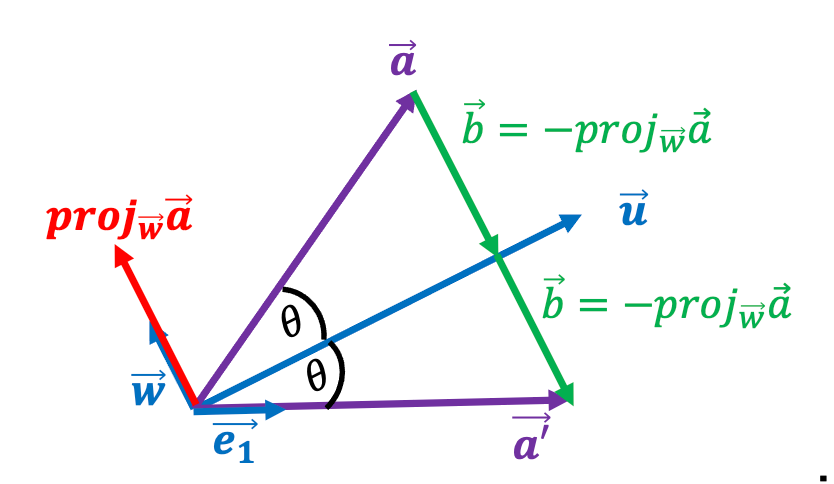
\includegraphics[width=1.0\textwidth]{Figures/householder.png}
    \caption{Primjer Householderove refleksije, preuzeto sa \cite{HouseholderSketch}}
    \label{fig:householder}
\end{figure}


\subsubsection{Svojstvena dekompozicija}
\label{sek:svojstvena_dekompozicija}
Svojstvena dekompozicija je implementirana kao metoda koja prima
kovarijacijsku matricu te par vlastitih vrijednosti i vlastitih vektora u koje
se spremaju rezultati dekompozicije.
Za izračun vlastitih vrijednosti koristi se \emph{metoda QR iteracija}
\cite{NLA} koja QR dekompoziciju
iterativno primjenjuje na matricu dok ne dobijemo i onda množi
matricu $R$ i $Q$ te tako dobivamo novu matricu koja je
približno dijagonalna. Zatim se vlastiti vektori dobivaju
posebno za svaku vlastitu vrijednost koristeći \emph{metodu
inverznih iteracija} \cite{NLA}. Ovakva implementacija nije
najefikasnija i sigurno među prvim optimizacijama koje bi se mogle
i trebale napraviti.




\subsection{Monte Carlo simulacija}
\label{sek:monte_carlo_simulacija}
\begin{figure}[H]
    \centering
    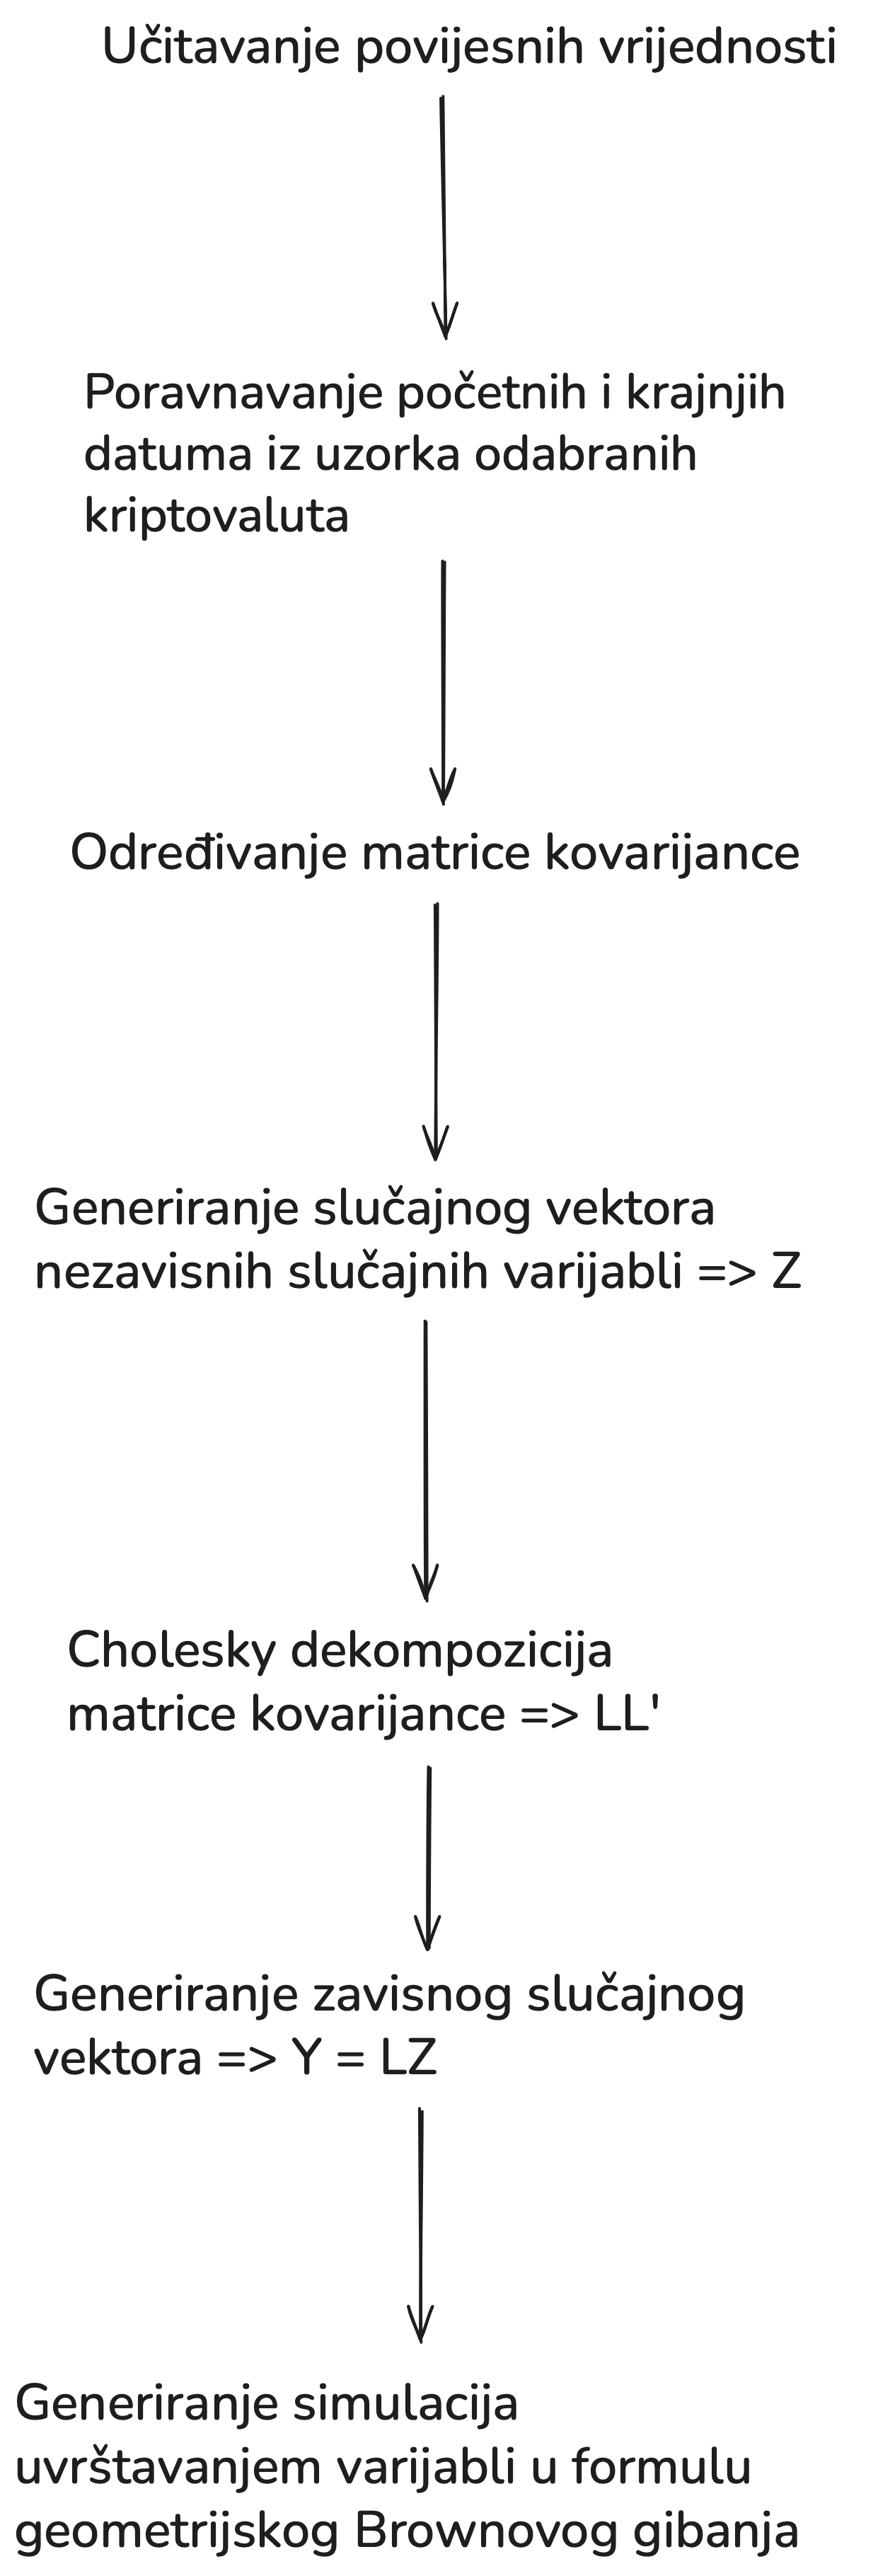
\includegraphics[height=0.7\textheight, keepaspectratio]{Figures/Monte_Carlo_explanation.png}
    \caption{Monte Carlo simulacija portfelja kriptovaluta}
    \label{fig:monte_carlo}
\end{figure}
Monte Carlo simulacija je implementirana kao metoda klase
\texttt{Portfolio} koja generira simulacije budućih cijena portfelja
kriptovaluta. Simulacije koriste model geometrijskog Brownovog gibanja
za generiranje budućih cijena te Cholesky dekompoziciju za
osiguranje uzoračke korelacije između kriptovaluta.
Implementacija Monte Carlo simulacija prvo koristi metodu za izračuvanje
kovarijacijske matrice portfelja iz povijesnih podataka kriptovaluta.
Također se može postaviti početni datum simulacije, broj simulacija i
broj koraka simulacije.
Zatim se koristeći \texttt{std::normal\_distribution(0,1)} generiraju
nezavisne slučajne varijable(\textasciitilde \textit{N(0,1)}) koje se
transformiraju u korelirane slučajne varijable pomoću Cholesky dekompozicije.
Zatim se ažuriraju cijene simulacije koristeći geometrijsko Brownovo gibanje
prema formuli:
\ref{sek:gbm}. Primjer rezultata simulacije je dan na slici
\ref{fig:monte_carlo_example}.
\begin{figure}[H]
    \centering
    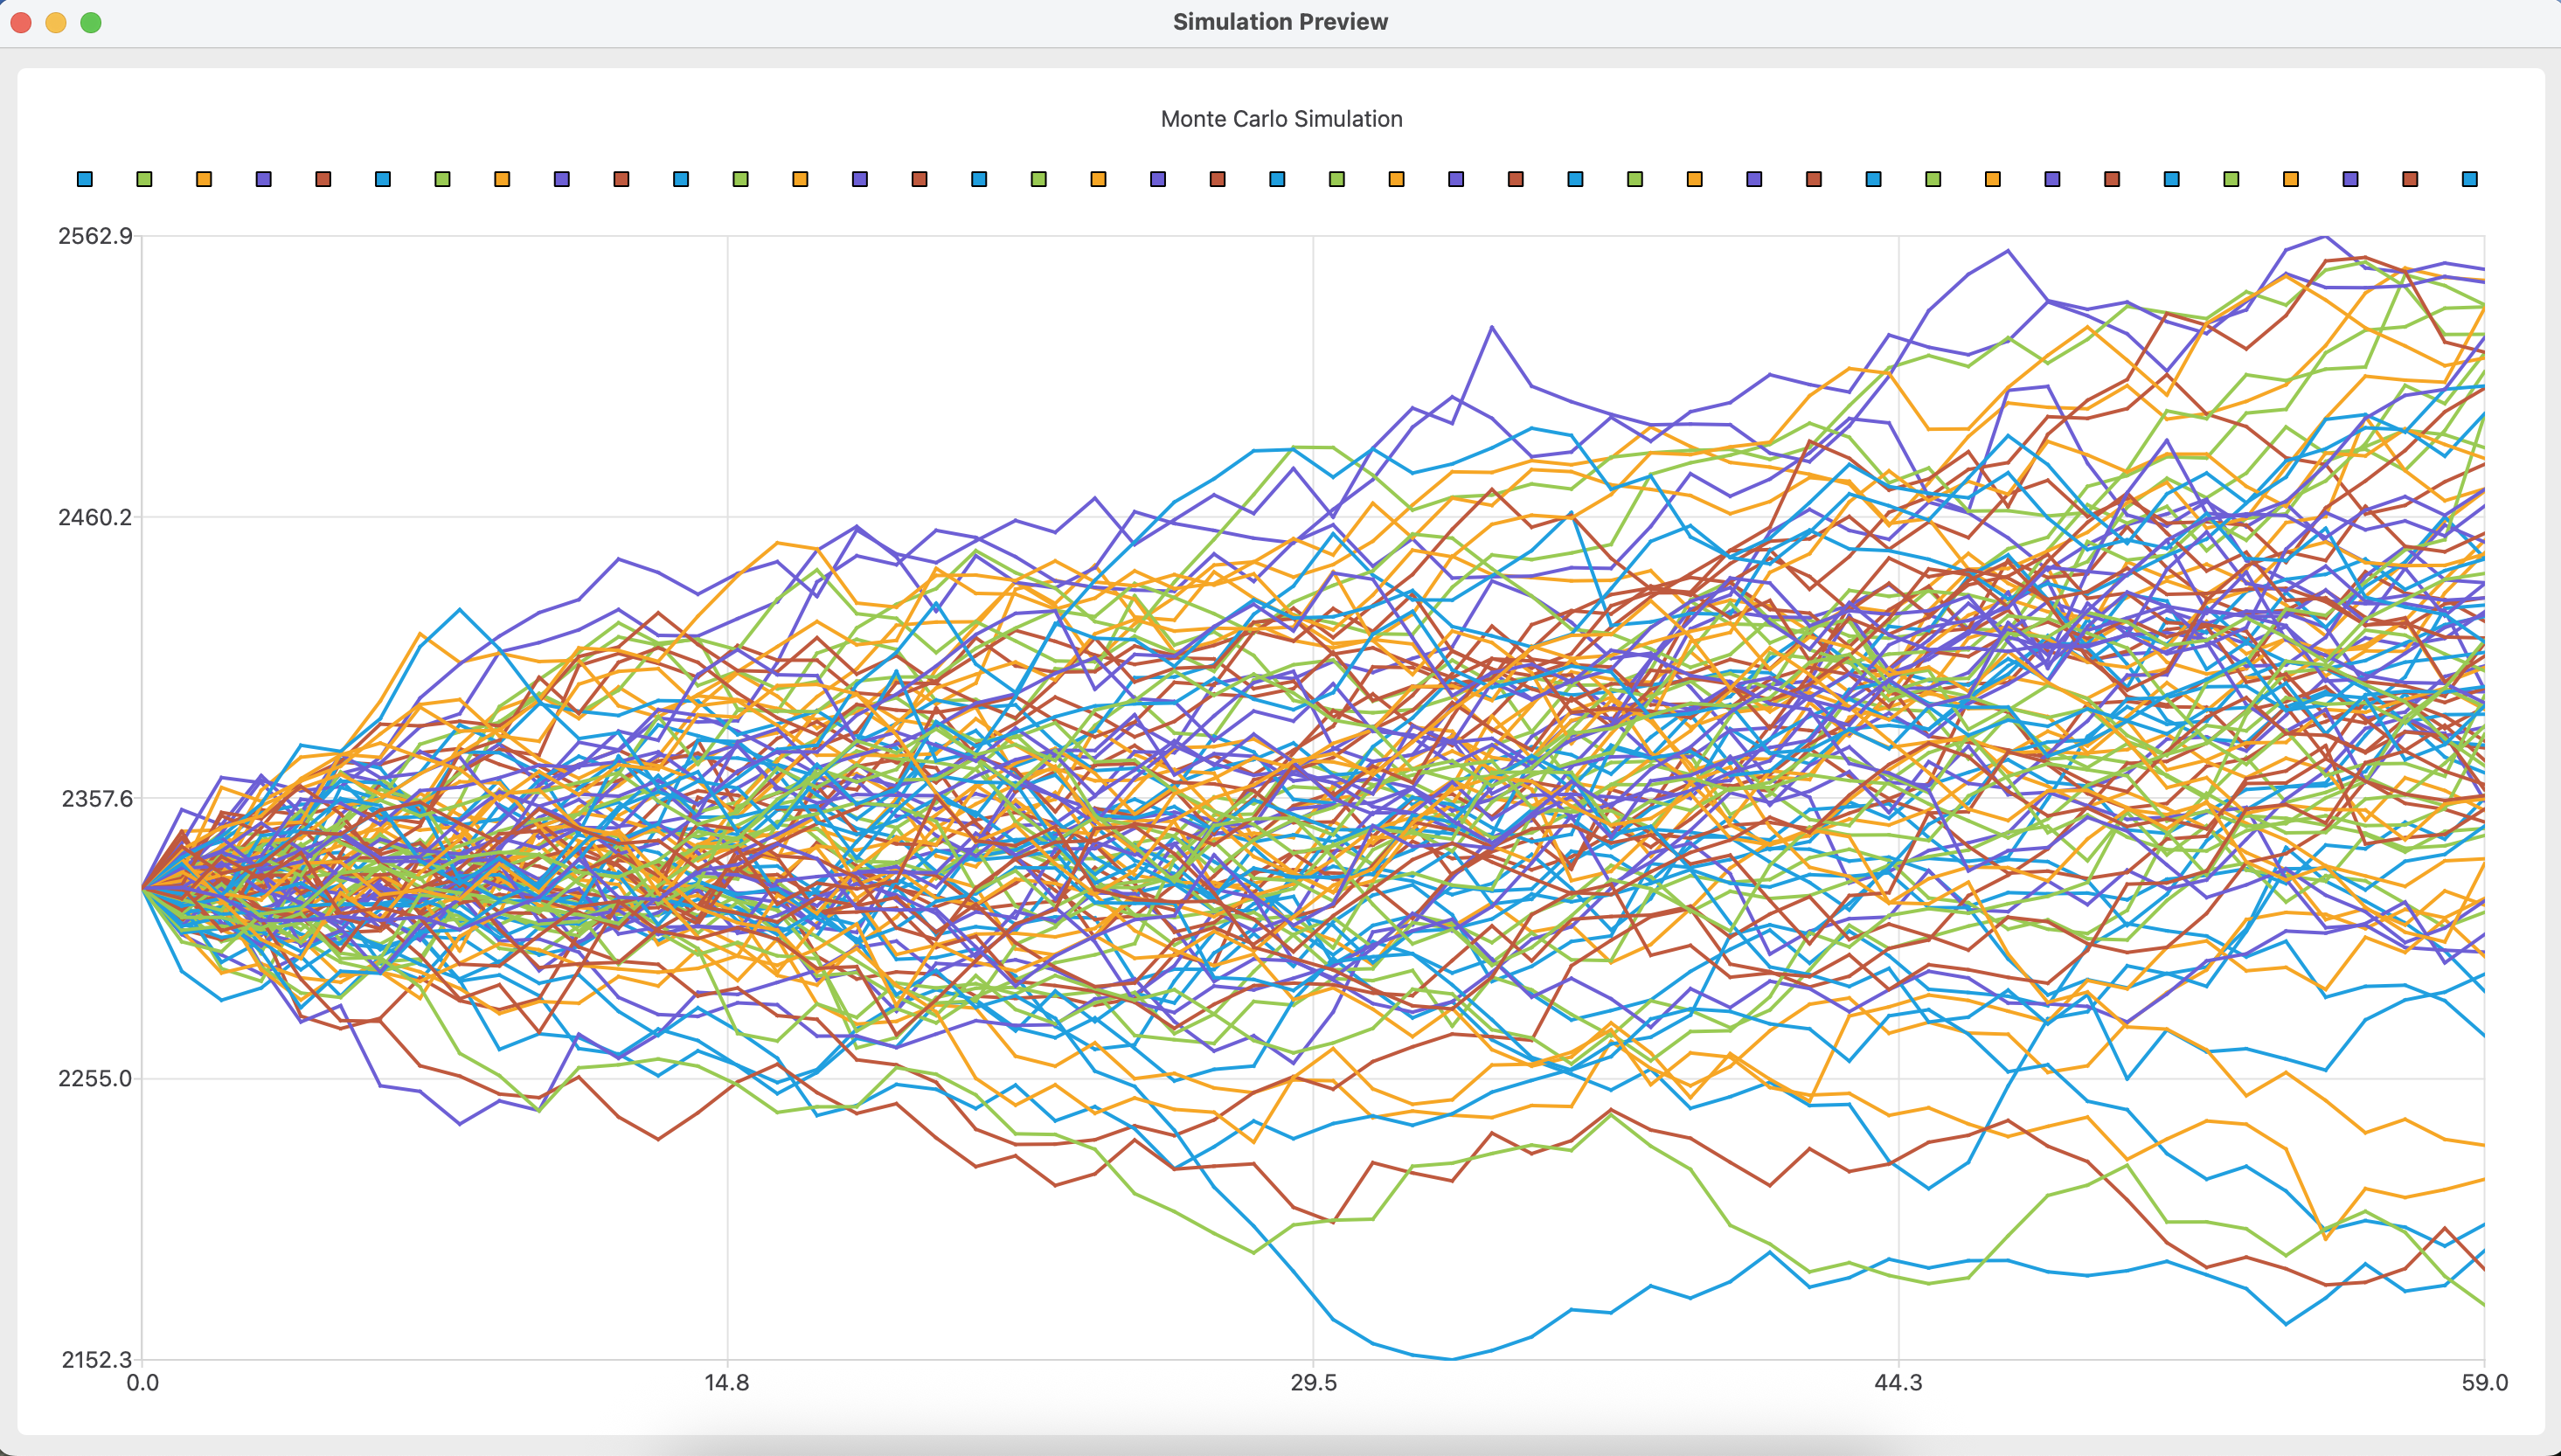
\includegraphics[width=1.0\textwidth]{Figures/monte_carlo_example.png}
    \caption{Primjer Monte Carlo simulacije portfelja kriptovaluta (100
    simulacija, 60 dana)}
    \label{fig:monte_carlo_example}
\end{figure}




\subsection{PCA dekompozicija}
\label{sek:pca_dekompozicija}
PCA dekompozicija je također implementirana kao metoda klase
\texttt{Portfolio} koja prima ulaznu kovarijacijsku matricu,
broj glavnih komponenti i vektor u koji se spremaju glavne komponente
poredane po količini varijance koju objašnjavaju te ukupnu varijancu (u ovom
slučaju to je suma svih vlastitih vrijednosti) i varijancu objašnjenu glavnim
komponentama. Metoda vrati \texttt{int} koji označava uspješnost dekompozicije.
Za izračun glavnih komponenti koristi se svojstvena dekompozicija koja
daje vlastite vrijednosti i vlastite vektore kovarijacijske matrice te je
objašnjena u \ref{sek:svojstvena_dekompozicija}.
primjer rezultata PCA dekompozicije je dan na slici
\ref{fig:pca_example}.
\begin{figure}[H]
    \centering
    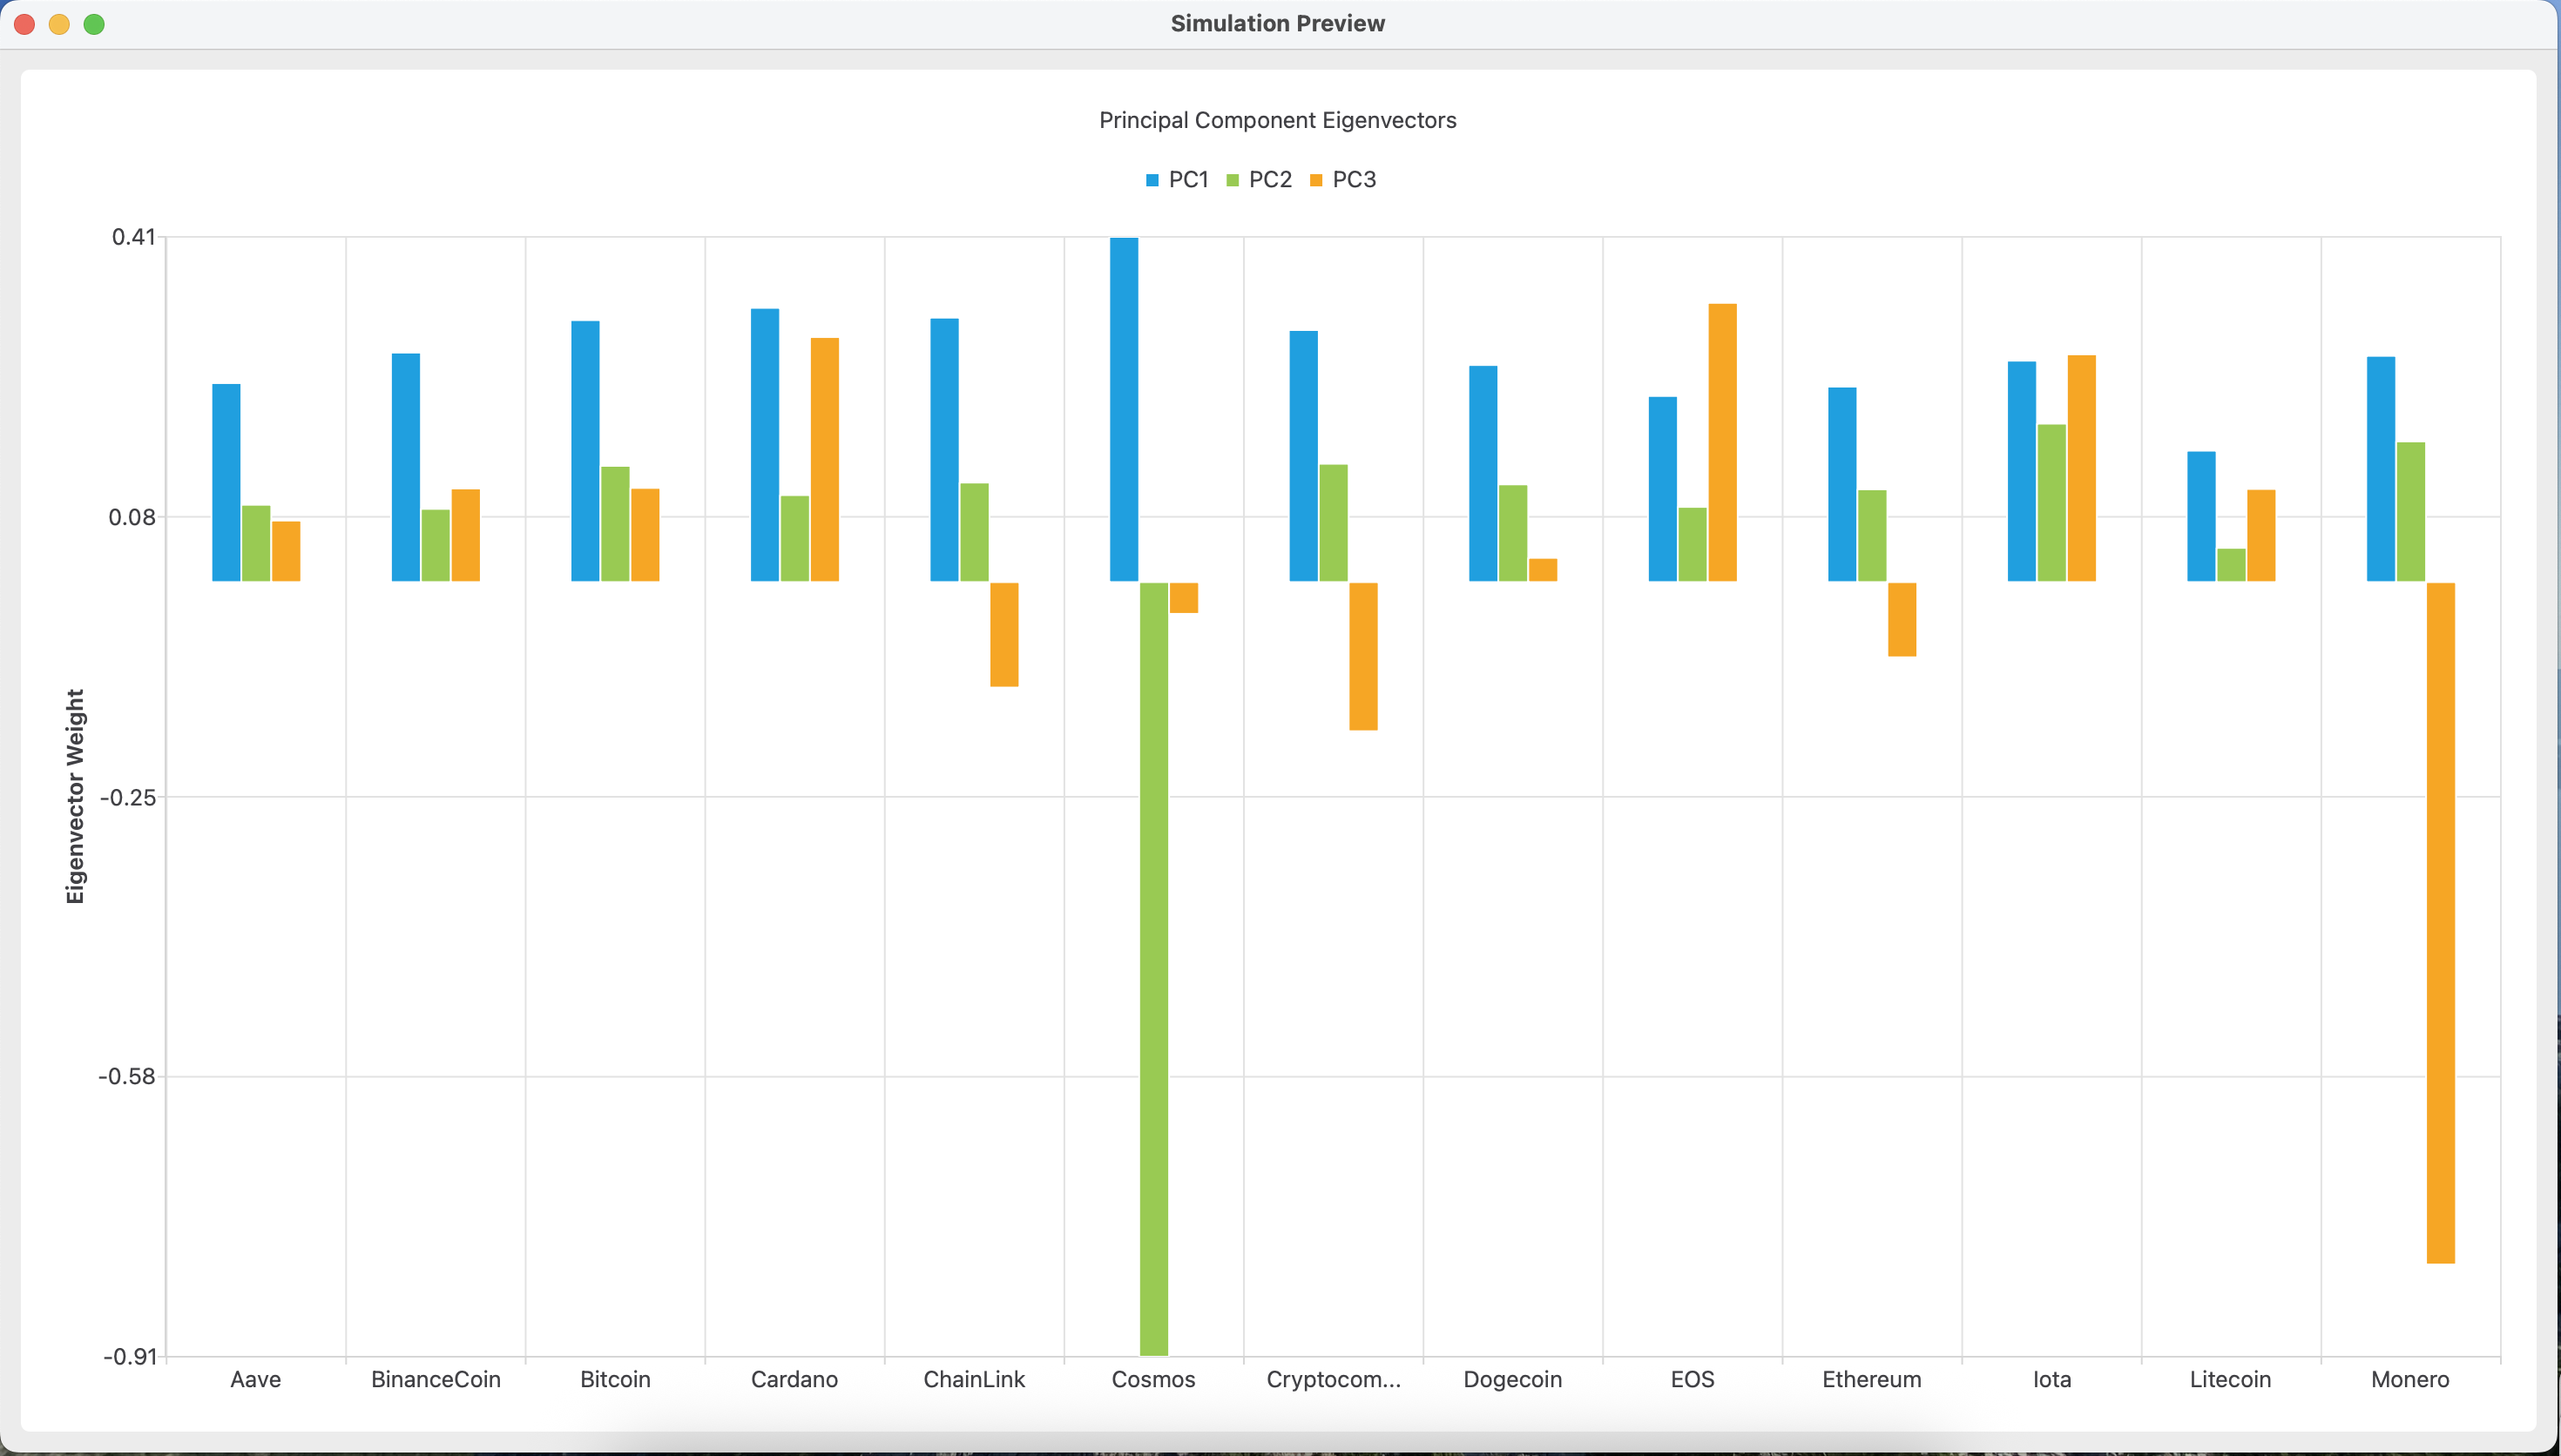
\includegraphics[width=1.0\textwidth]{Figures/pca_example.png}
    \caption{Primjer PCA dekompozicije portfelja kriptovaluta (3 glavne komponente)}
    \label{fig:pca_example}
\end{figure}

\subsection{Vizualizacija rezultata}
\label{sek:vizualizacija_rezultata}
Za vizualizaciju rezultata i interakciju s korisnikom koristi se
grafičko sučelje implementirano u \texttt{C++} koristeći Qt biblioteku.
Grafičko sučelje omogućuje korisniku da odabere kriptovalute koje želi
staviti u portfelj, postavi udjele kriptovaluta u portfelju,
odabere vremenski period simulacije i broj simulacija.
Rezultati simulacija se prikazuju u obliku grafova koji
se otvaraju u novom prozoru aplikacije i prikazuju teoretsko kretanje
vrijednosti portfelja u budućnosti. Korisnik također može odabrati
broj glavnih komponenti te izvrši PCA dekompoziciju portfelja. Prikaz
rezultata PCA dekompozicije je također u obliku grafova koji
se otvara u novom prozoru aplikacije i prikazuje glavne komponente
portfelja te varijancu koju objašnjavaju.
\begin{figure}[H]
    \centering
    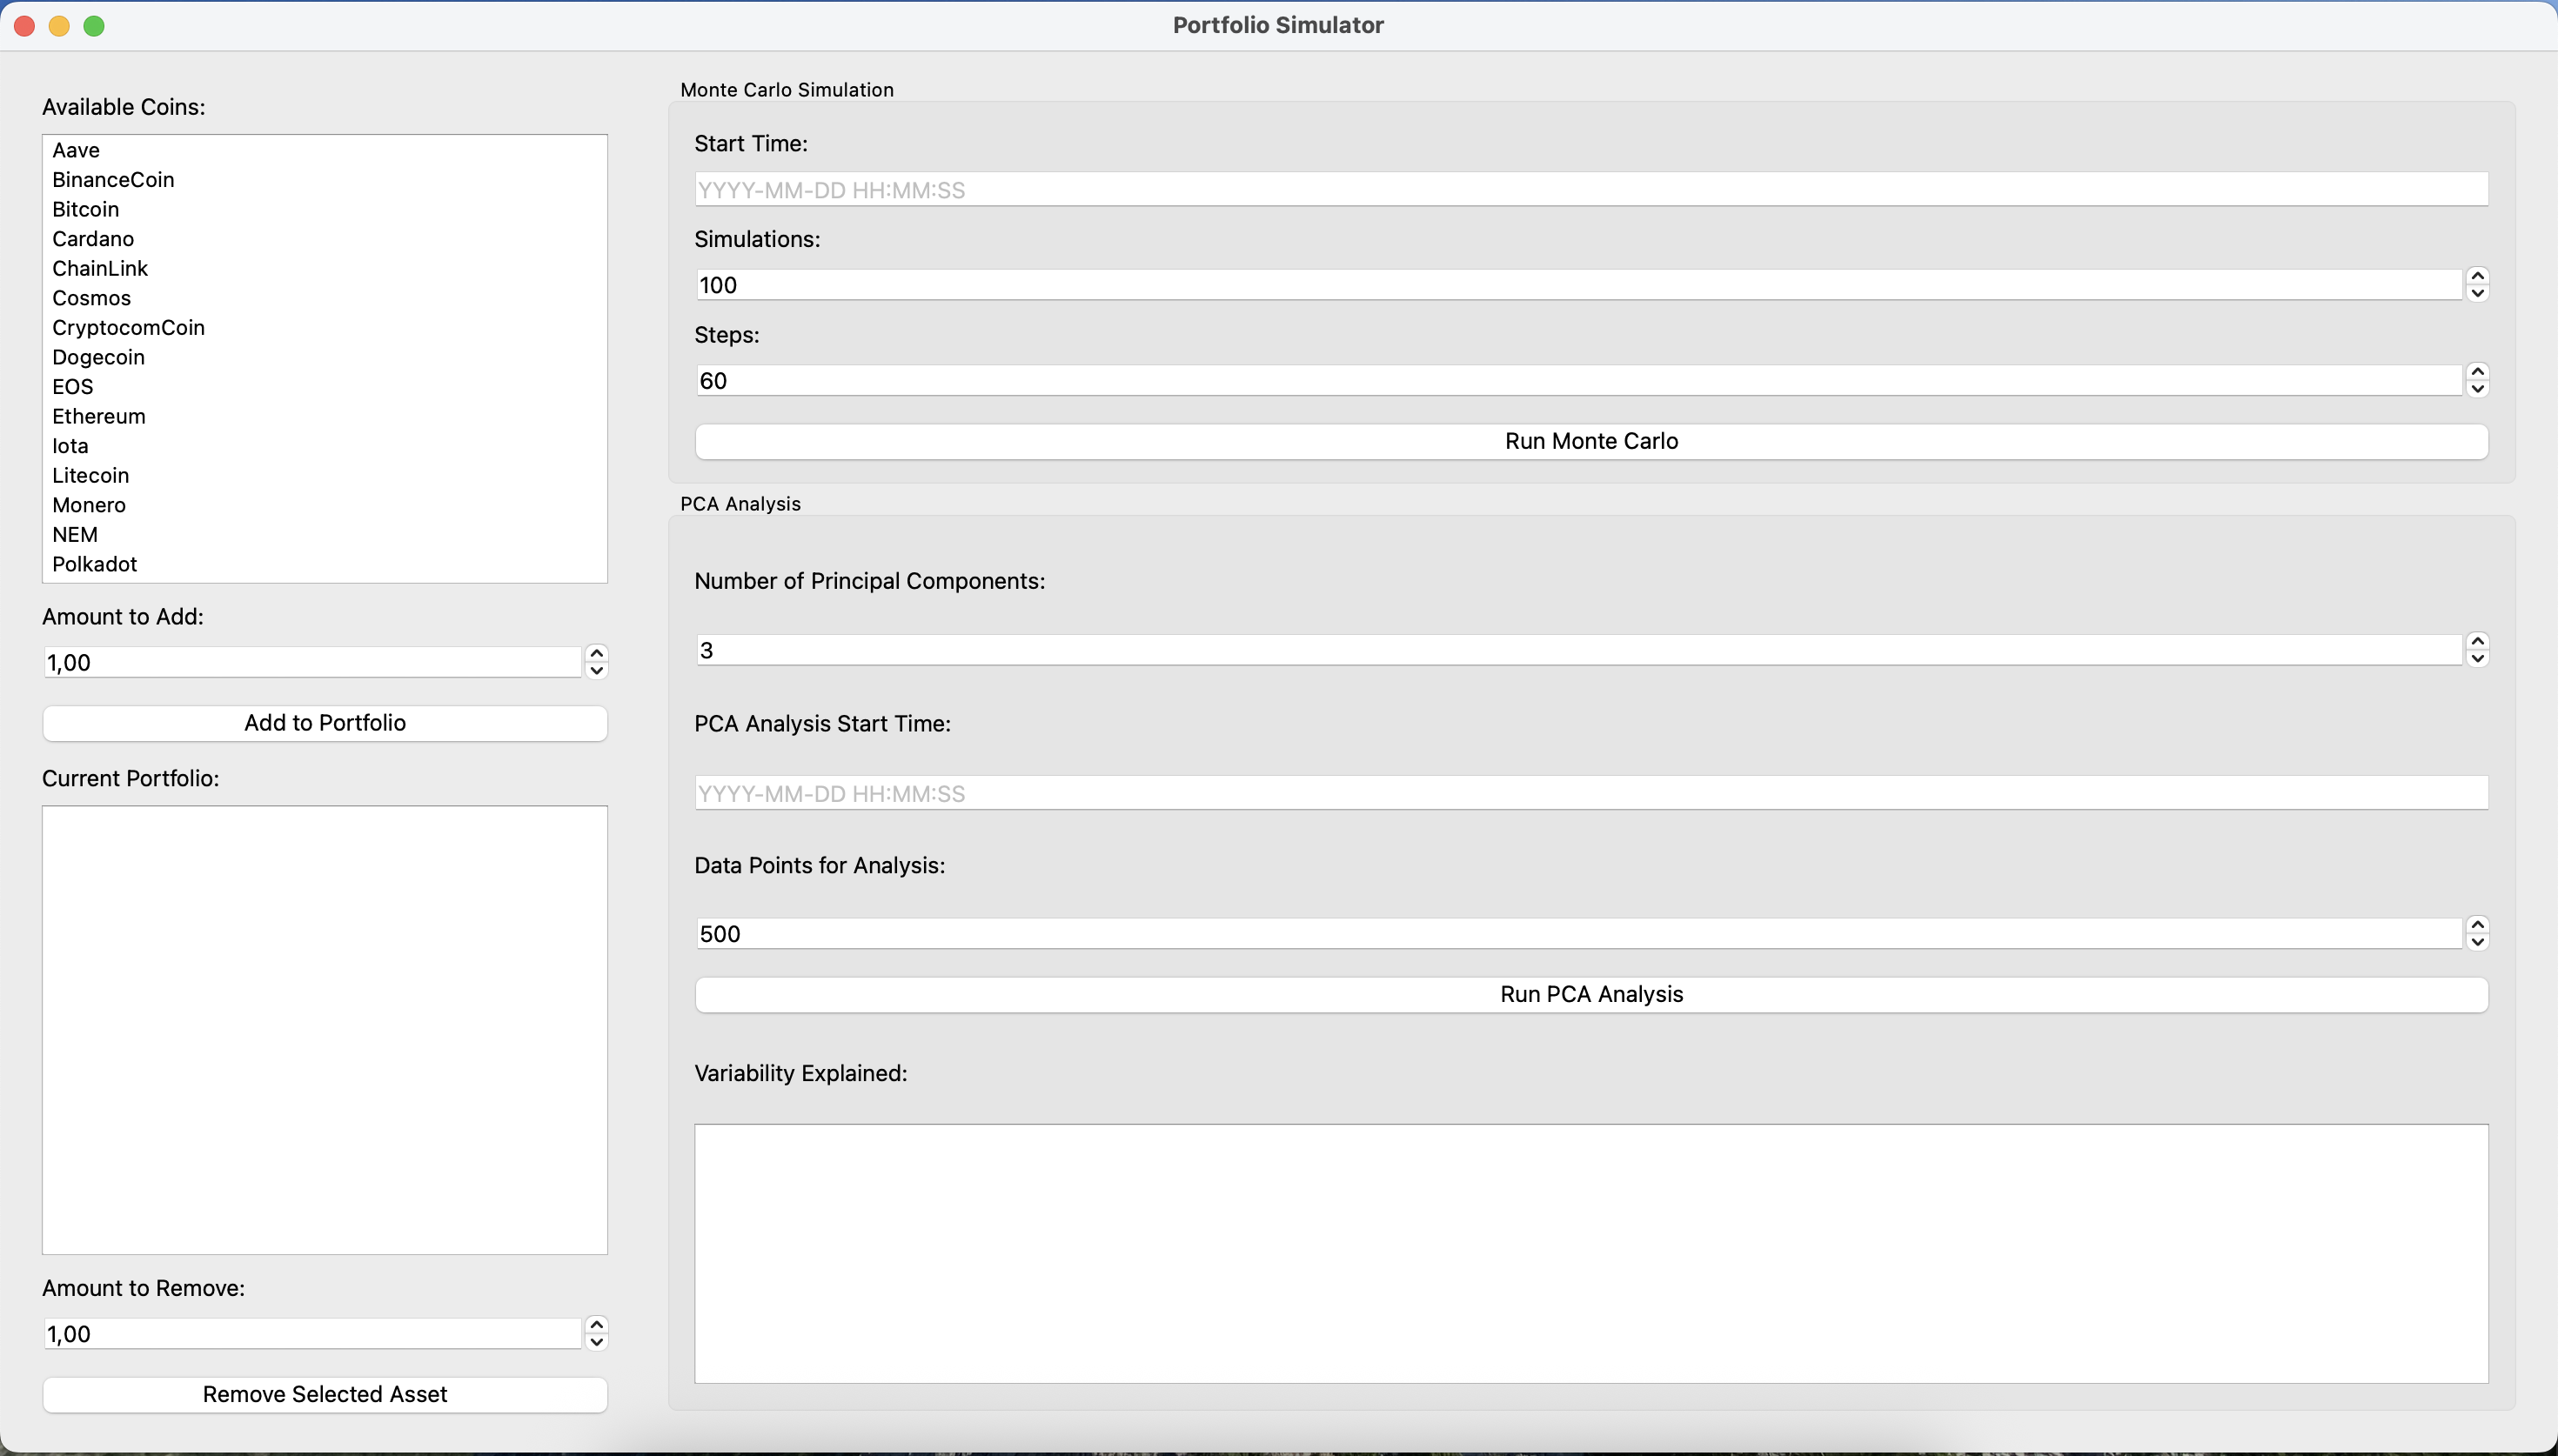
\includegraphics[width=1.0\textwidth]{Figures/gui.png}
    \caption{Grafičko sučelje aplikacije za simulaciju portfelja kriptovaluta}
    \label{fig:portfolio_gui}
\end{figure}

% Rasprava
\chapter{Rezultati i rasprava}
\label{pog:rezultati_i_rasprava}
U ovom poglavlju prikazujemo rezultate postignute implementacijom aplikacije
te raspravljamo o njihovoj važnosti i primjenjivosti u stvarnom svijetu.
Također, analiziramo prednosti i nedostatke implementacije te mogućnosti
optimizacija i proširenja aplikacije.
\section{Analiza i diskusija implementacijskih rezultata}
\label{sek:implementacijski_rezultati}
\subsection{Funkcionalnost učitavanja i parsiranja podataka}
Ručna implementacija parsiranja podataka omogućila je
optimizaciju učitavanja i obrade podataka zbog specifičnosti
izgleda samog skupa podataka. Osim što odmah znamo koji su stupci
prisutni dodatna optimizacija je postignuta pregledavanjem veličine
datoteke i aproksimacijom broja redaka u datoteci. To nam omogućuje
da unaprijed rezerviramo memoriju za vektor \emph{candle} struktura
što značajno ubrzava proces parsiranja pogotovo kod većih skupova
podataka jer ne moramo konstantno realocirati memoriju pri proširivanju
vektora. Ova implementacija je na dostpunim skupovima podataka
postigla brzinu parsiranja usporedivu s popularnom bibliotekom
\emph{csv2} \cite{csv2} koja je optimizirana za parsiranje CSV datoteka.

\subsection{Matematički okvir}
\label{sek:matematicki_okvir_rezultati}
Matematički okvir aplikacije implementiran je tako da
se koristi samo standardna biblioteka \texttt{C++}. Iako je ovakav pristup
produljio vrijeme izrade aplikacije te samo izvođenje aplikacije
nije optimizirano kao što bi bilo da se koriste biblioteke poput
\emph{Eigen} \cite{Eigen3} ili \emph{Armadillo} \cite{10980539},
koje koriste optimizirane algoritme i strukture podataka za
matematičke operacije te napredne optimizacije poput \emph{SIMD} instrukcija,
\emph{template metaprogramming}-a i \emph{expression templates}-a,
ovakav pristup je omogućio dublje razumijevanje i primjenu
stečenih znanja.\\
Implementacija se specifično oslanja
na \texttt{std::vector} kao osnovnu strukturu podataka za vektore i
matrice. \texttt{std::vector} je dinamički niz koji omogućuje
efikasno upravljanje memorijom i automatsko proširivanje
kada je potrebno.\\
Većina matematičkih operacija je implementirana na \emph{naivni} način
kako bi se osiguralo da su svi koraci jasni i razumljivi. Jedine
optimizacije su napravljene koristeći \emph{move semantics} i
kako bi se izbjeglo nepotrebno kopiranje podataka te korištenje
\texttt{OpenMP}-a \cite{660313} za paralelizaciju određenih operacija.
Sve operacije su testirane na skupnjenim skupovima podataka i
vrijeme izvođenja je zadovoljavajuće za većinu operacija. Jedino
što je potrebno optimizirati je traženje vlastitih vektora koristeći
neki od asimptotski efikasnijih algoritama u odnosu na \emph{metodu
inverznih iteracija}.

\subsection{Monte Carlo simulacija}
\label{sek:monte_carlo_rezultati}
Monte Carlo simulacija se pokazala kao efikasan način
generiranja vjerojatnosnih scenarija budućih cijena portfelja kriptovaluta
ukoliko je inicijalni uzorak smislen i dovoljno velik.
Jedan primjer simulacije koji izgleda realistično i smislen je
dan je ranije na slici \ref{fig:monte_carlo_example}.
Na tom se primjeru vidi blagi pozitivni \textit{drift} cijena portfelja
te volatilnost koja je u skladu s očekivanjima za portfelj kriptovaluta.
\\
Drugi primjer simulacije je dan na slici \ref{fig:monte_carlo_example2}.
\begin{figure}[H]
    \centering
    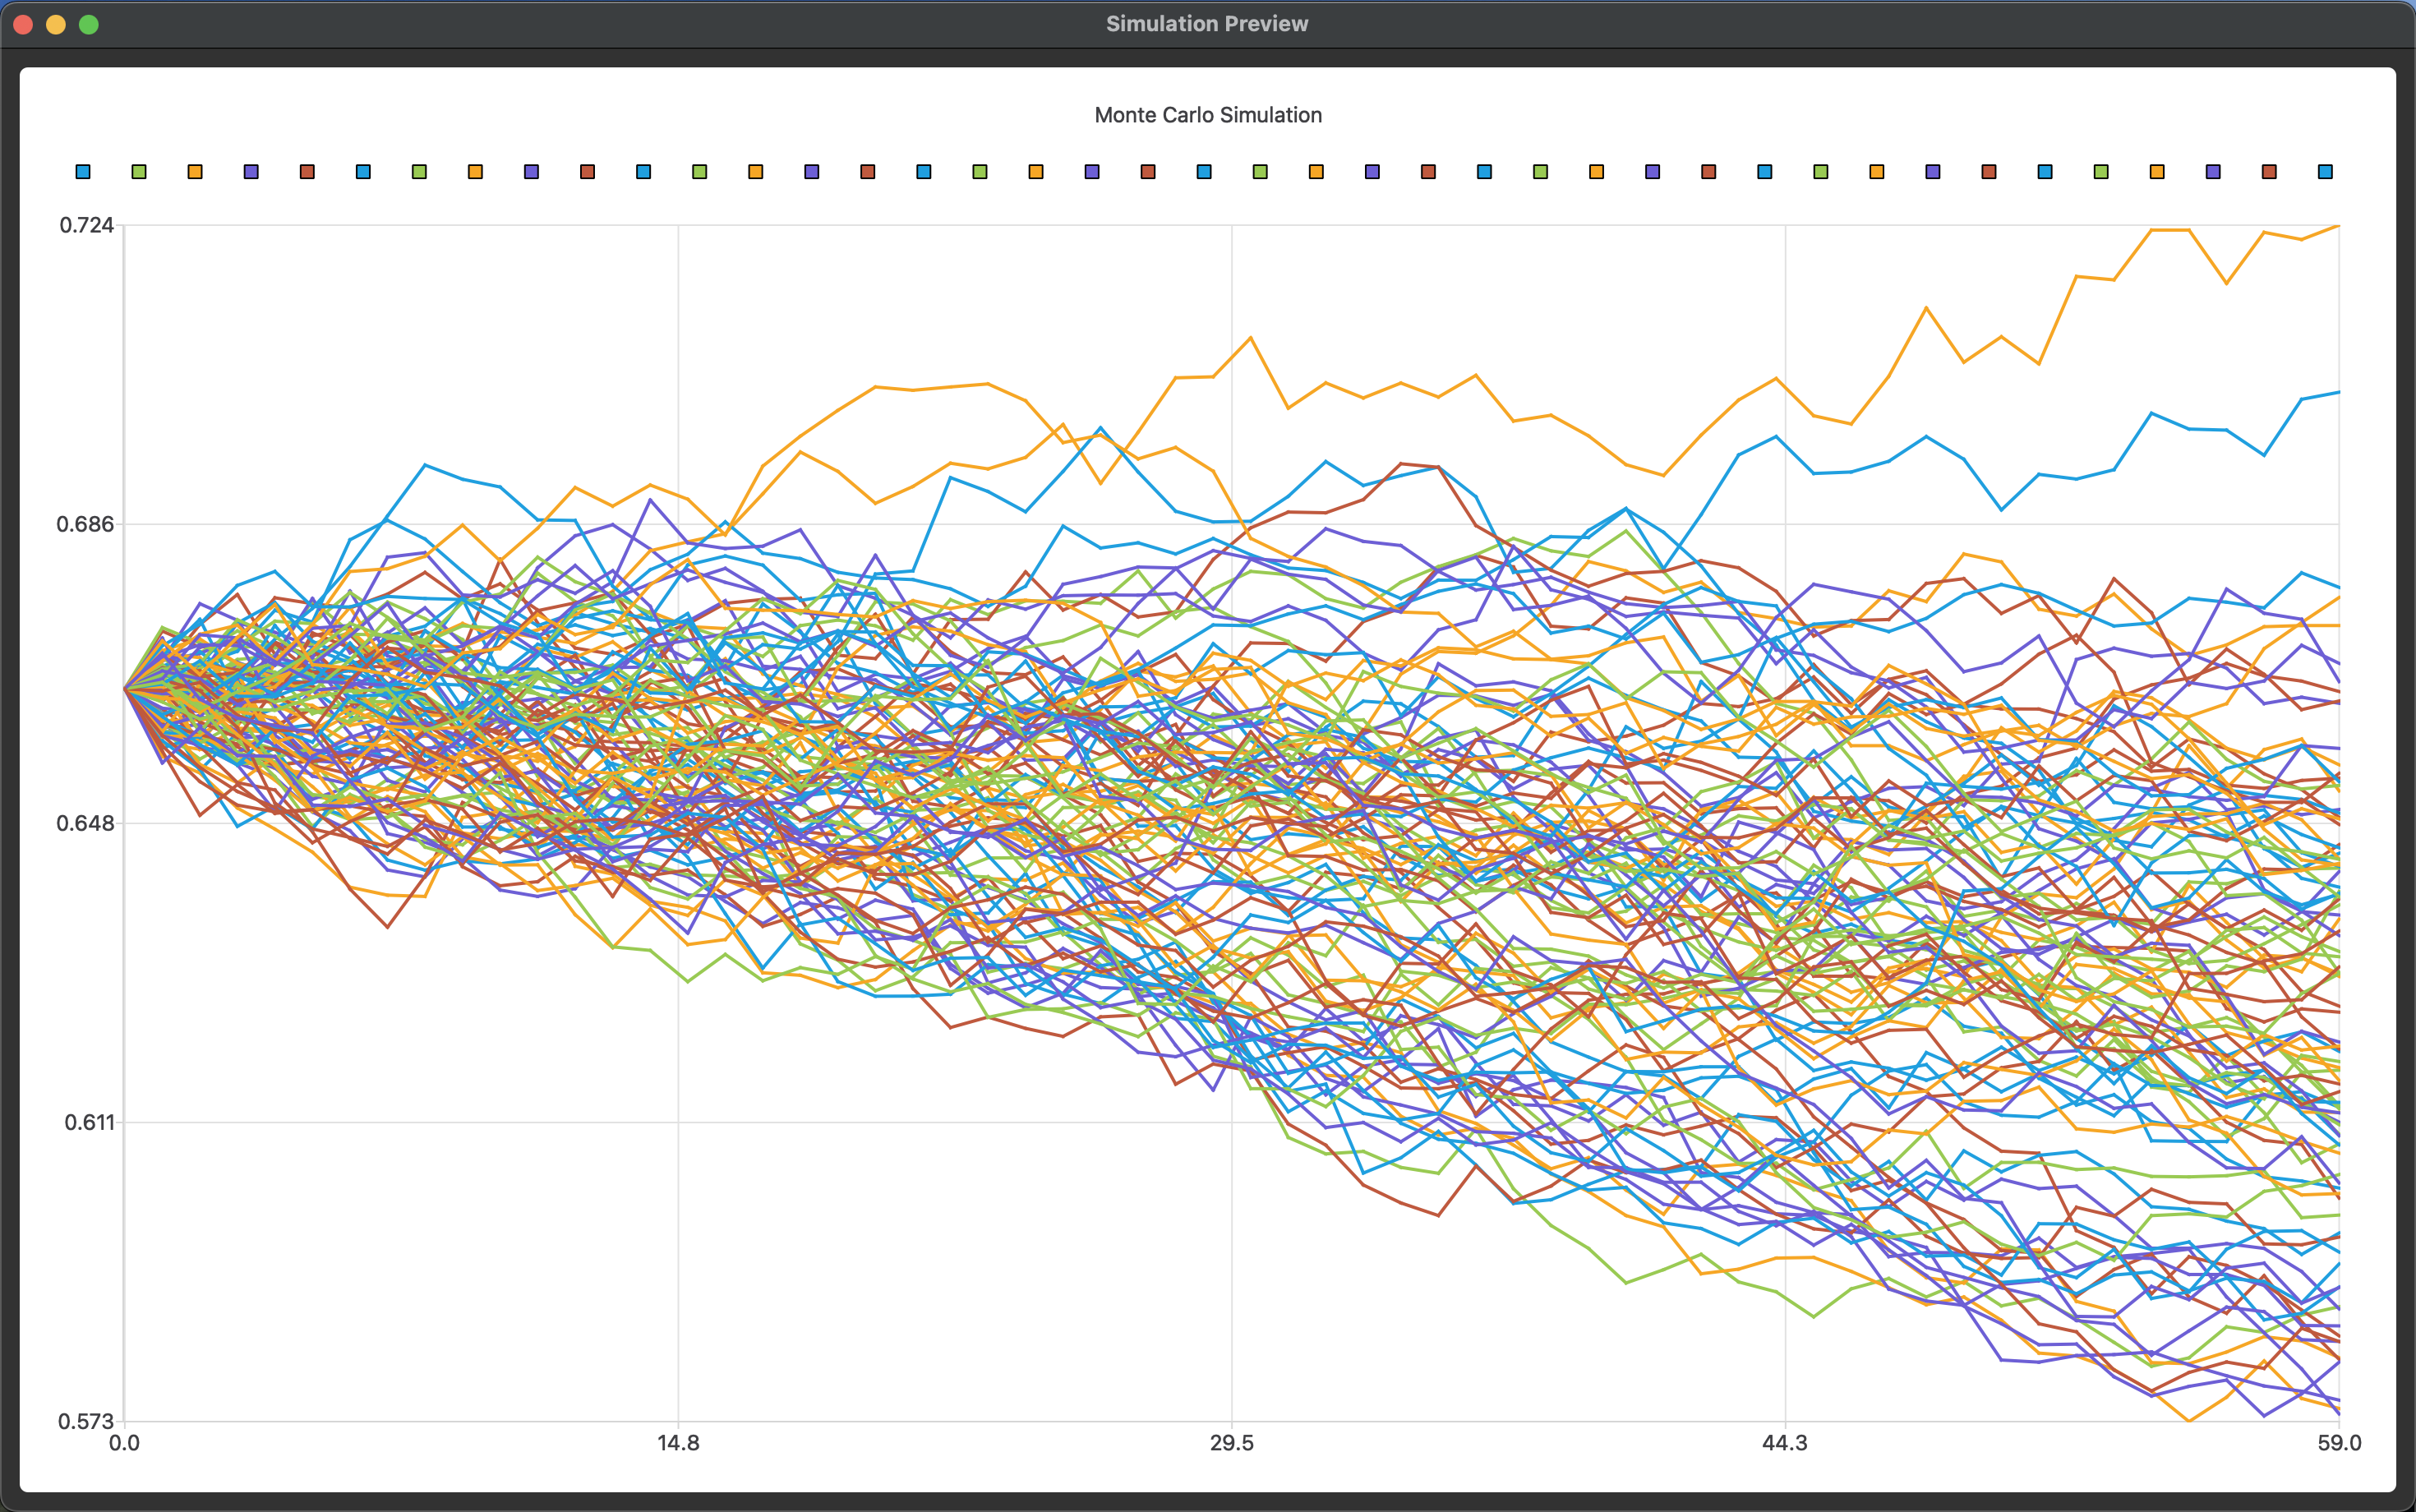
\includegraphics[width=1.0\textwidth]{Figures/monte_carlo_example2.png}
    \caption{Primjer Monte Carlo simulacije portfelja (XRP) kriptovaluta (100
    simulacija, 60 dana)}
    \label{fig:monte_carlo_example2}
\end{figure}

Ovaj primjer simulacije pokazuje da je \textit{drift} cijena portfelja
negativan, ali da je volatilnost portfelja također visoka. Ovakav
izgled simulacije je očekivan ako uzmemo u obzir da koristimo
statističku metodu koja gleda samo povijesne podatke i ne uzima u obzir
puno drugih faktora koji utječu na cijene kriptovaluta. Izgled kretanja
vrijednosti portfelja u povijesnim podatcima dan je na slici \ref{fig:XRP_hist}.
Na slici se vidi da je volatilnost cijene kriptovalute XRP
visoka te je vrijednost iste u zadnjih nekoliko godina
većinom opadala uz 2 velika i nagla porasta.
\begin{figure}[H]
    \centering
    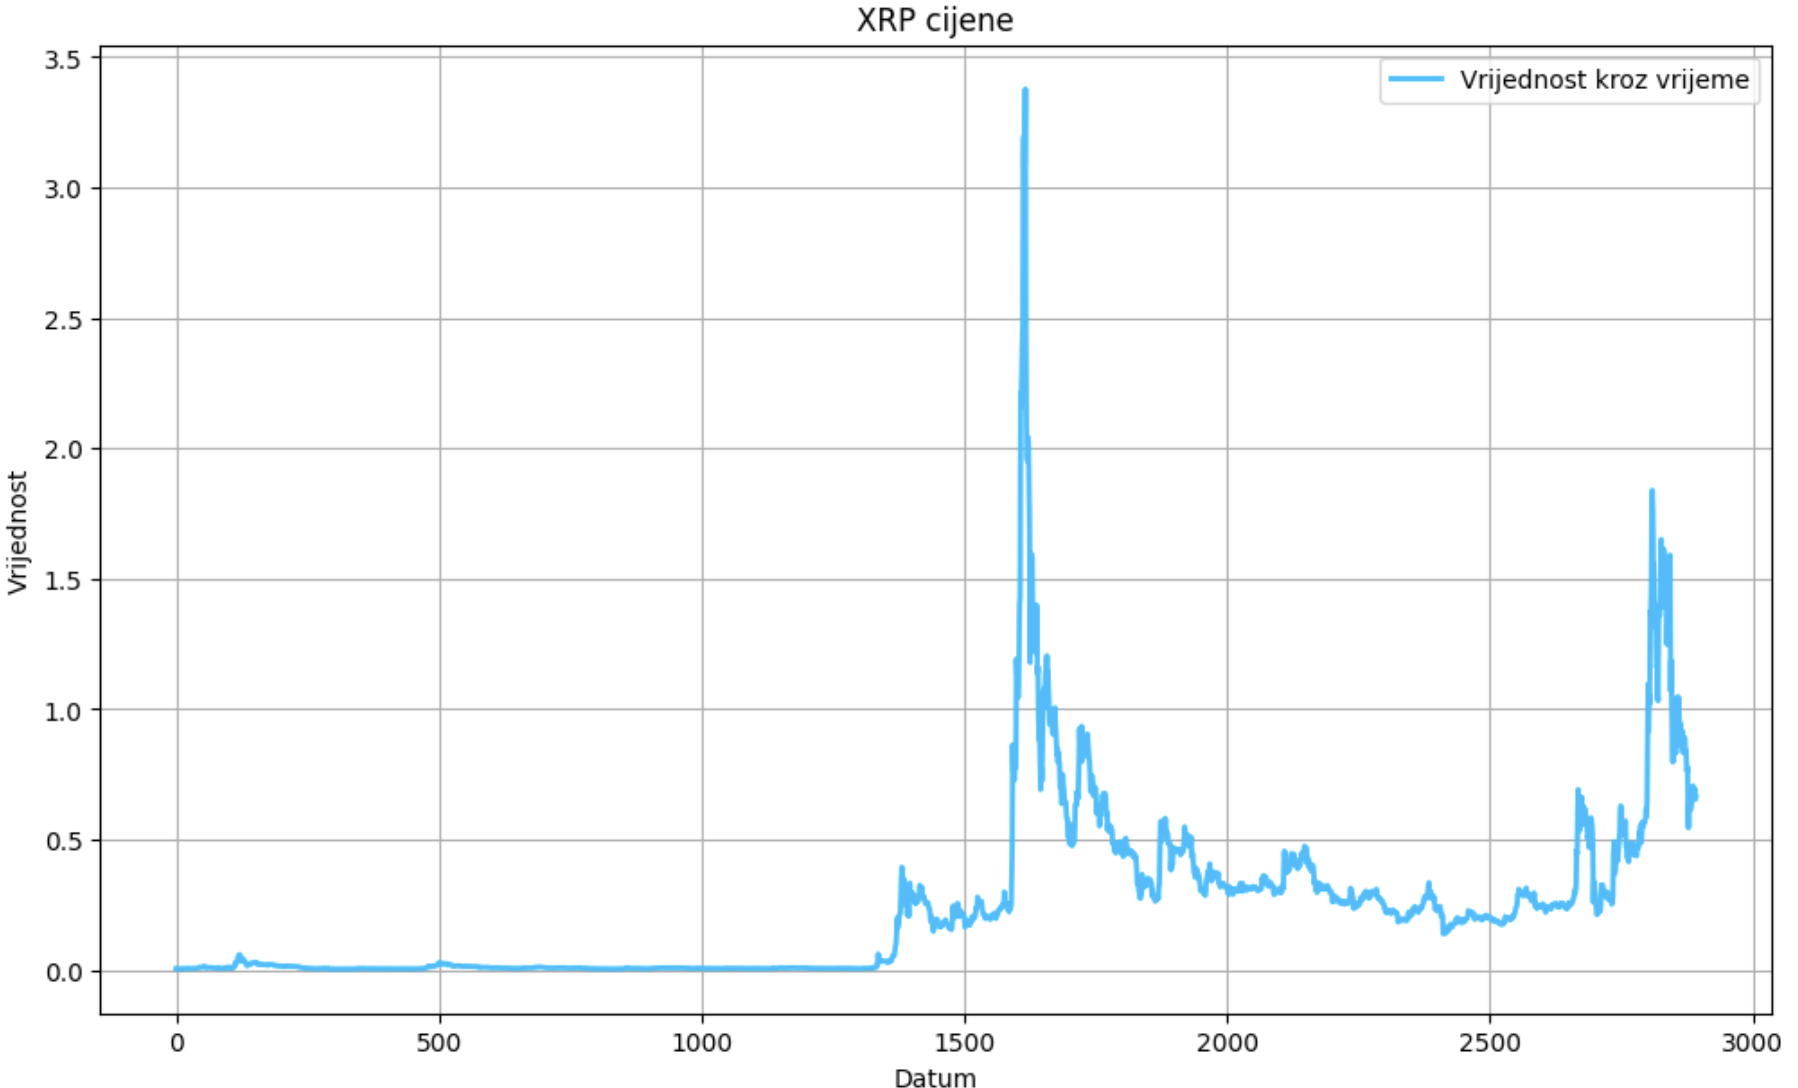
\includegraphics[width=1.0\textwidth]{Figures/XRP_hist.png}
    \caption{Povijesno kretanje cijene kriptovalute XRP}
    \label{fig:XRP_hist}
\end{figure}

Treći primjer simulacije je dan na slici \ref{fig:monte_carlo_example3}.
Na slici se vidi da je \textit{drift} cijena portfelja poprilično
pozitivna, ali da je volatilnost opet visoka.\\
U ovom primjeru uočavamo problem kod Monte Carlo simulacija za
kriptovalute. Budući da se o finacijskim instrumentima koji su
relativno novi i malo je povijesnih podataka,
Monte Carlo simulacije koje su statistička metoda i temelje se
na povijesnim podacima, ne daju uvijek
realistične rezultate bez uzimanja u obzir dodatnih informacija o tržištu.
Iz ove bi se simulacije moglo zaključiti da očekujemo rast vrijednosti
od nekoliko posto u sljedećih 60 dana, ali to nije nužno točno
(iako je vrijednost \textit{Bitcoin}-a stvarno značajno porasla u proteklom vremenu).
Također je uz toliko pozitivan \textit{drift} i volatilnost teško
dobro odrediti jer utjecaj \textit{drift}-a u samoj formuli
\ref{sek:gbm} je dovoljno značajan da model neće predvidjeti kroz
toliki period vremena da će vrijednost portfelja pasti.
\begin{figure}[H]
    \centering
    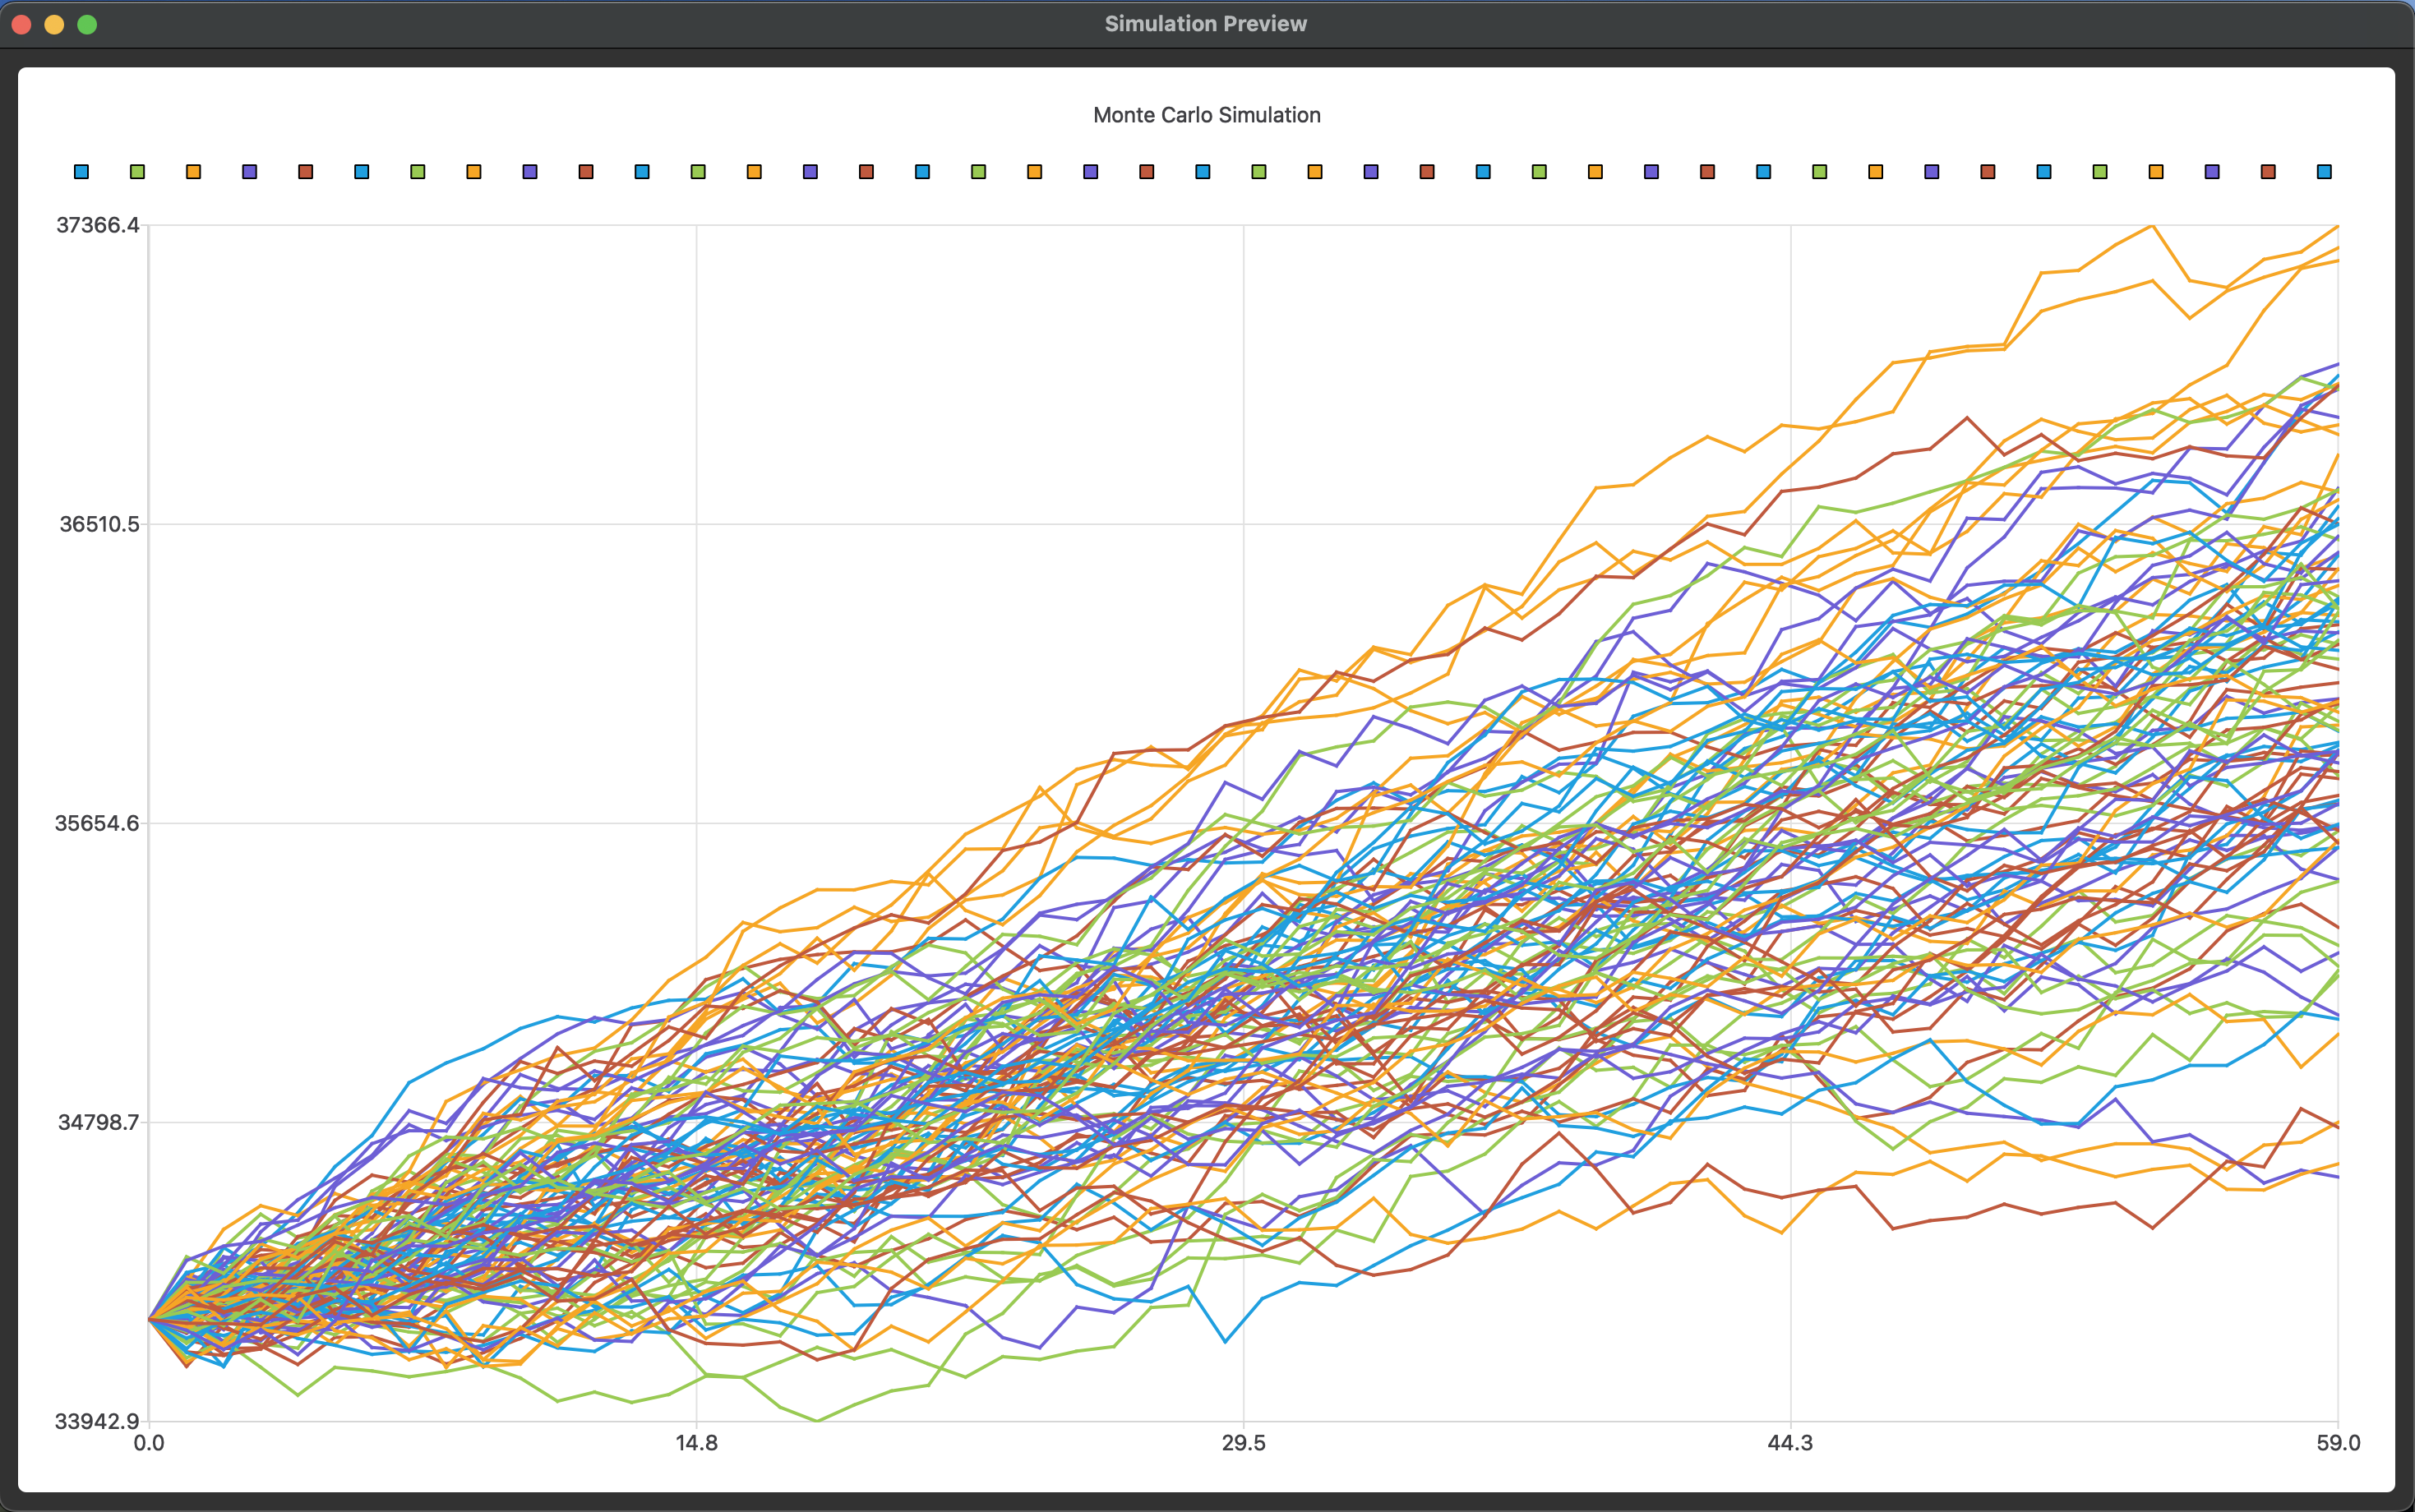
\includegraphics[width=1.0\textwidth]{Figures/monte_carlo_example3.png}
    \caption{Primjer Monte Carlo simulacije portfelja (Bitcoin) kriptovaluta (100
    simulacija, 60 dana)}
    \label{fig:monte_carlo_example3}
\end{figure}
Promatajući povijesne podatke \textit{Bitcoin}-a, dane na slici \ref{fig:BTC_hist},
vidimo da je volatilnost cijene \textit{Bitcoin}-a također visoka, ali da je
zapravo cijena \textit{Bitcoin}-a u zadnjih nekoliko godina većinom snažno
rasla uz nekoliko manjih padova. Ovakav izgled povijesnih podataka
zapravo potpuno opravdava pozitivni \textit{drift} i sam izgled
simulacije u \ref{fig:monte_carlo_example3}.
\begin{figure}[H]
    \centering
    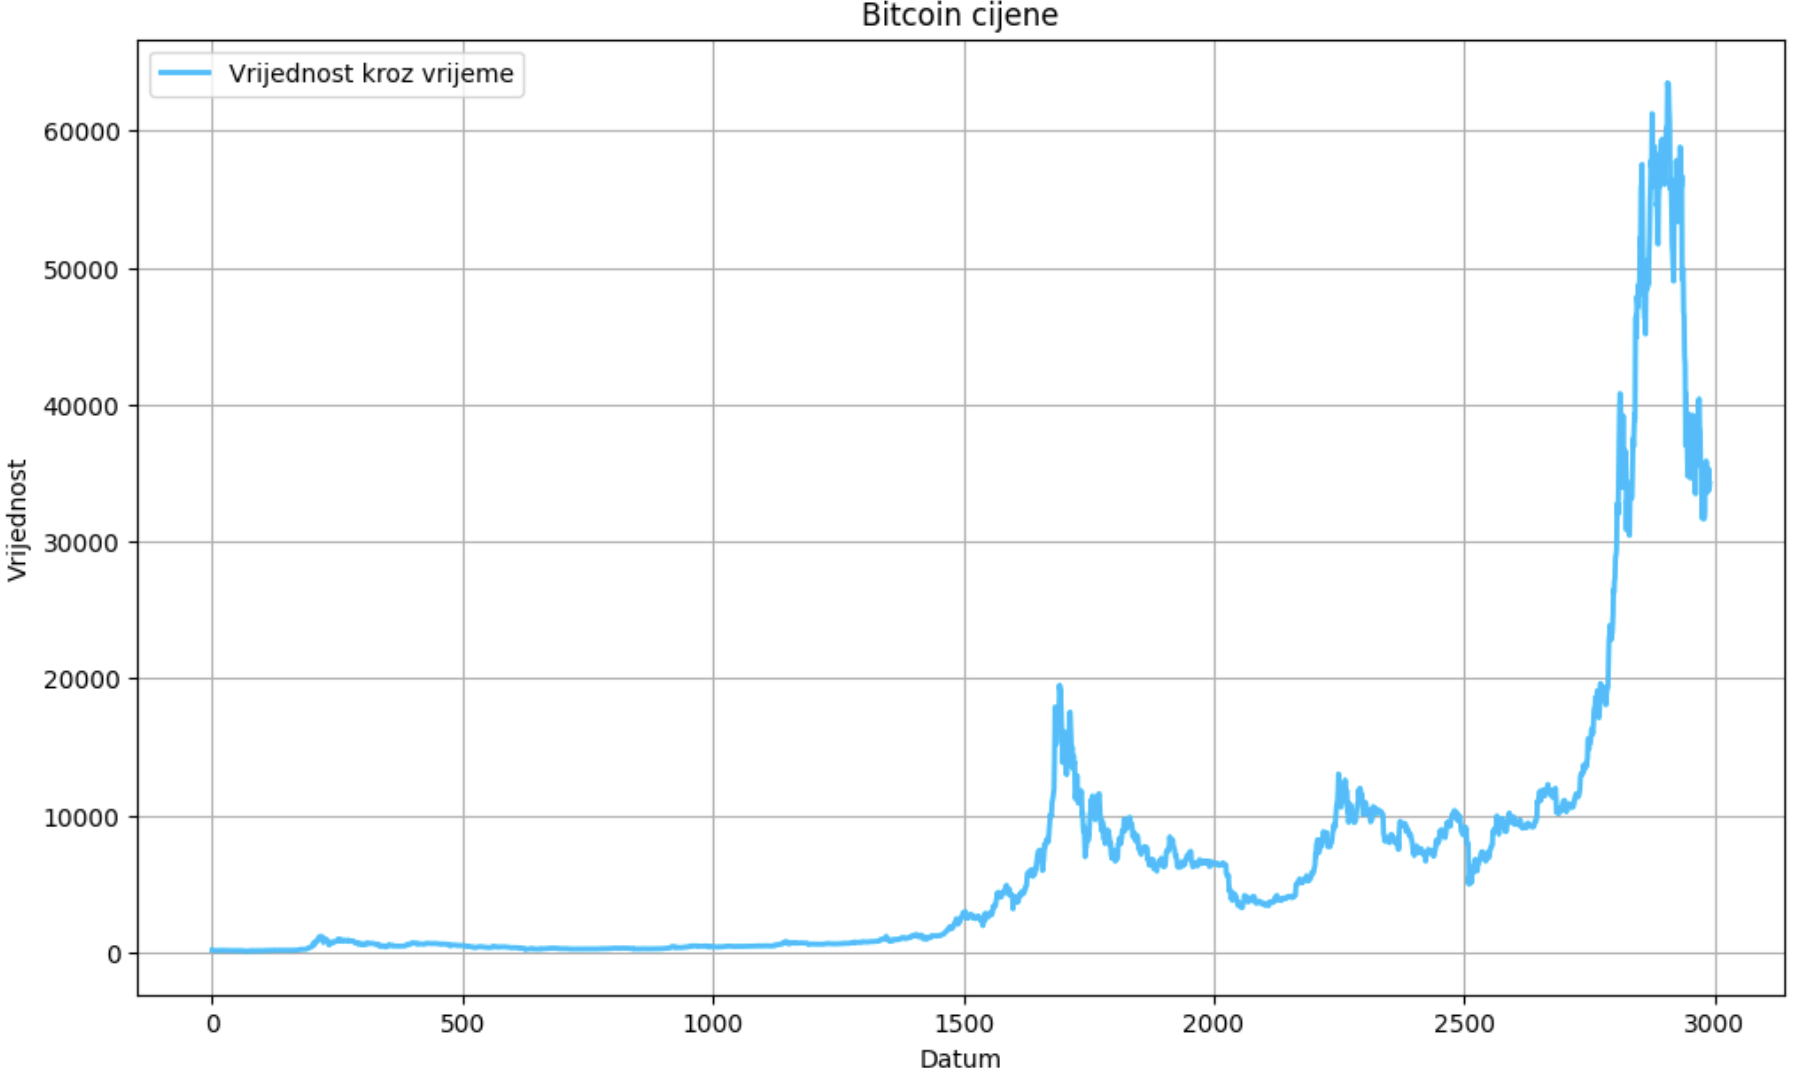
\includegraphics[width=1.0\textwidth]{Figures/BTC_hist.png}
    \caption{Povijesno kretanje cijene kriptovalute Bitcoin}
    \label{fig:BTC_hist}
\end{figure}


\subsection{PCA dekompozicija}
\label{sek:pca_rezultati}

Implementacija PCA dekompozicije koristi implementirane metode
za izračunavanje uzoračke kovarijacijske matrice te nakon toga poziva
metoda za određivanje svojstvenih vrijednosti i vektora. To zapravo znači
da je većina vremena izvođenja ovisna o implementaciji svojstvene dekompozicije
jer je asimptotski najsporija od svih operacija. Kao što je ranije spomenuto,
implementacija koristi \emph{metodu QR iteracija} za izračun svojstvenih
vrijednosti
i \emph{metodu inverznih iteracija} za izračun svojstvenih vektora.
Ovakva implementacija je dovoljno brza za manje skupove podataka i za
potrebe ove aplikacije, ali već za matrice veličine 30x30 i više
vrijeme izvođenja je par sekundi što je neprihvatljivo za
aplikaciju koja bi trebala raditi u realnom vremenu. Ovakva bi se
implementacija trebala optimizirati korištenjem i pametnijih algoritama
za izračun svojstvenih vrijednosti i vektora te optimizacijama na
razini \texttt{C++} koda, kao što su \emph{SIMD} instrukcije i \emph{Cache}
optimizacije.\\
Primjer rezultata PCA dekompozicije je dan na slici \ref{fig:pca_example}.
Iz tog i sljedećeg primjera danog na slici \ref{fig:pca_example2}
se vidi da su kriptovalute jako međusobno korelirane i može se primijetiti
da je prva glavna komponenta zapravo svojstveni portfelj približno
jednakih težina.
\begin{figure}[H]
    \centering
    \includegraphics[width=1.0\textwidth]{Figures/pca_example2.png}
    \caption{Primjer PCA dekompozicije portfelja kriptovaluta (3 glavne komponente)}
    \label{fig:pca_example2}
\end{figure}

\subsection{Vizualizacija rezultata}
\label{sek:vizualizacija_rezultata_rezultati}
Grafičko sučelje aplikacije omogućuje korisnicima jednostavno
upravljanje portfeljem, pokretanje simulacija i vizualizaciju rezultata.
Vizualizacija rezultata simulacija i PCA dekompozicije
omogućuje korisnicima bolje razumijevanje rizika i mogućnosti portfelja
kriptovaluta. Grafovi su interaktivni i omogućuju korisnicima
da pregledavaju rezultate simulacija i PCA dekompozicije na različite načine.
Implementacija grafičkog sučelja je napravljena korištenjem Qt biblioteke
koja omogućuje jednostavno kreiranje grafičkog sučelja i apstrakciju
od niskorazinskih detalja upravljanja prozorima i događajima.
Iako je ovakvo rješenje dovoljno dobro za potrebe ove aplikacije,
u budućnosti bi se mogla razmotriti implementacija ručnog rješenja
za grafičko sučelje kako bi se dobila veća fleksibilnost i kontrola
nad izgledom i ponašanjem sučelja. Također, mogla bi se razmotriti
izrada boljeg rješenja za vizualizaciju rezultata simulacija i PCA dekompozicije
kao što su 3D grafovi ili animacije koje bi omogućile bolje razumijevanje
rizika i mogućnosti portfelja kriptovaluta.\\
Navedena poboljšanja bi omogućila također i bolji dizajn aplikacije
te unaprijeđenje korisčkog iskustva u vidu \textit{UX} i \textit{UI} dizajna.

\chapter{Upute za korištenje i pokretanje aplikacije}
\label{sek:upute_za_koristenje}
Aplikacija se može pokrenuti na bilo kojem sustavu koji podržava
\texttt{C++} i \texttt{Qt} biblioteku. Potrebno je instalirati \texttt{Qt}
biblioteku na lokalno računalo te imati dostupan \texttt{Clang} kompilator.
Nakon toga se može ili ručno kompajlirati aplikacija koristeći dani
\texttt{CMakeLists.txt} unutar direktorija \texttt{App} ili se može
pokrenuti \texttt{build\_script.sh} skripta koja je također unutar direktorija
\texttt{App} i automatski stvara izvršnu datoteku aplikacije. Skripta je
napisana za \texttt{Unix} okruženje.
Nakon kompajliranja aplikacije unutar direktorija \texttt{App/build} će se
stvoriti izvršna datoteka \texttt{PortfolioSimulator} koja se može pokrenuti
direktno iz terminala. Aplikacija će se pokrenuti u grafičkom sučelju
i korisnik dalje može interaktivno koristiti aplikaciju. Uz samu aplikaciju
stvara se i dodatna datoteka \texttt{run\_tests} koja služi za provođenje
testova aplikacije. Testovi su napisani opet u \texttt{C++} i koriste samo standardnu
biblioteku \texttt{C++}. Napisani su tako da pokrivaju sve ključne
komponente aplikacije i provjeravaju ispravnost implementacije.
Sve naredbe i primjeri za pokretanje aplikacije i testova dani su u
nastavku.
\begin{lstlisting}[language=bash, caption={Primjeri naredbi za pokretanje aplikacije i testova}]
# Kloniranje repozitorija
git clone https://github.com/IvanDzanija/PortfolioSimulator.git
# Pozicioniranje u direktorij aplikacije
cd PortfolioSimulator/App
# Pokretanje skripte za kompajliranje aplikacije
./build_script.sh
# Pokretanje aplikacije
./build/PortfolioSimulator
# Pokretanje testova
./build/run_tests
\end{lstlisting}




%--- ZAKLJUČAK / CONCLUSION ----------------------------------------------------
\chapter{Zaključak}
\label{pog:zakljucak}
U ovom radu prikazan je razvoj aplikacije za modeliranje investicijskih
portfelja kriptovaluta korištenjem Monte Carlo simulacija
i PCA dekompozicije. Kroz teorijski pregled objašnjeni su ključni
financijski i matematički koncepti poput teorije portfelja, modela
geometrijskog Brownovog gibanja, kovarijacijske matrice,
Cholesky i PCA dekompozicije, čime je postavljen temelj za razumijevanje
i implementaciju modela. Implementacija je realizirana u \texttt{C++} programskom
jeziku, uz korištenje standardne biblioteke i vlastitih rješenja za
matematičke operacije, što je omogućilo detaljno razumijevanje svakog
koraka i fleksibilnost u razvoju.
Rezultati pokazuju da Monte Carlo simulacije omogućuju generiranje
vjerojatnosnih scenarija budućih vrijednosti portfelja, ali i ukazuju na
ograničenja povezana s visokom volatilnošću i kratkom poviješću kriptovaluta.
PCA dekompozicija dodatno je omogućila redukciju dimenzionalnosti i
identifikaciju glavnih izvora rizika u portfelju, pri čemu su rezultati
potvrdili visoku međusobnu koreliranost kriptovaluta. Analiza
funkcionalnosti aplikacije pokazala je da je ručna implementacija
parsiranja i matematičkog okvira bila dovoljno brza i pouzdana za manje
skupove podataka, ali bi za veće skupove i rad u realnom vremenu bilo
potrebno dodatno optimizirati algoritme, osobito algoritam za izračun svojstvenih
vrijednosti i vektora.
Aplikacija, uz grafičko sučelje, omogućuje korisnicima jednostavno
upravljanje portfeljem, pokretanje simulacija i vizualizaciju rezultata,
što može pomoći u boljem razumijevanju i upravljanju rizicima povezanima s
kriptovalutama. Ograničenja modela proizlaze iz oslanjanja na povijesne
podatke i pretpostavke o distribuciji i parametrima procesa, zbog čega rezultati
simulacija ne mogu u potpunosti predvidjeti buduće tržišne događaje.

Tijek daljnjeg razvoja aplikacije bi uključivao integraciju naprednijih
statističkih modela koji nisu toliko ovisni o početnoj pretpostavci
distribucije i parametara, proširenje podrške za \textit{real-time}
podatke te optimizacija postojećih algoritama korištenjem specijaliziranih
matematičkih algoritama i optimizacijom prisupa \textit{Cache} memoriji.
Razvijeni programski okvir i biblioteka za rad s
financijskim podacima mogu poslužiti kao temelj za buduća istraživanja i
razvoj naprednijih alata u području financijske analitike i upravljanja
rizikom te svojom modularnošću pružiti dodatni edukacijski resurs.

%--- LITERATURA / REFERENCES ---------------------------------------------------

% Literatura se automatski generira iz zadane .bib datoteke / References are automatically generated from the supplied .bib file
% Upiši ime BibTeX datoteke bez .bib nastavka / Enter the name of the BibTeX file without .bib extension
\bibliography{literatura}

%--- SAŽETAK / ABSTRACT --------------------------------------------------------

% Sažetak na hrvatskom
\begin{sazetak}
    ``PortfolioSimulator`` je aplikacija za modeliranje investicijskih
    portfelja kriptovaluta korištenjem Monte Carlo simulacija i PCA
    dekompozicije. Aplikacija je implementirana u \texttt{C++} programskom jeziku,
    koristeći standardnu biblioteku \texttt{STL} i vlastita rješenja za
    matematičke, matrične i vektorske operacije te \texttt{Qt} biblioteku
    za grafičko sučelje.
    Povijesni podaci o cijenama 23 kriptovalute preuzeti su s
    javno dostupnog izvora, a korisniku je omogućeno upravljanje
    portfeljem i simulacijama.
    U uvodnom dijelu objašnjeni su ključni financijski i matematički
    koncepti: teorija portfelja, geometrijsko Brownovo gibanje,
    kovarijacijska matrica, Cholesky i PCA dekompozicija.
    Analiza rezultata pokazuje da su kriptovalute visoko međusobno
    korelirane i volatilne, što ograničava preciznost modela
    temeljenih isključivo na povijesnim podacima.
    U sljedećem poglavlju detaljno je opisana implementacija svega
    potrebnog za rad aplikacije, uključujući parsiranje podataka,
    matematički okvir, modele kriptovaluta i portfelja te Monte Carlo
    simulacije i PCA dekompoziciju. Na kraju je dan pregled postignutih
    rezultata, rasprava o funkcionalnosti aplikacije i upute za korištenje
    i pokretanje.
\end{sazetak}

\begin{kljucnerijeci}
    PortfolioSimulator; Monte Carlo simulacije; PCA dekompozicija;
    kriptovalute; \texttt{C++}; Qt; STL; stohastički modeli; financijska analitika;
\end{kljucnerijeci}

% Abstract in English
\begin{abstract}
    "PortfolioSimulator" is an application for modeling
    investment portfolios of cryptocurrencies using Monte Carlo
    simulations and PCA decomposition. The application is implemented
    in the \texttt{C++} programming language, utilizing the standard library
    \texttt{STL}
    and custom solutions for mathematical, matrix, and vector operations,
    as well as the \texttt{Qt} library for the graphical interface.
    Historical price data for 23 cryptocurrencies were obtained from a
    publicly available source, and the user is able to manage the
    portfolio and simulations.
    The introductory section explains key financial and mathematical
    concepts: portfolio theory, geometric Brownian motion, covariance
    matrix, Cholesky and PCA decomposition.
    The analysis of the results shows that cryptocurrencies are highly
    intercorrelated and volatile, which limits the accuracy of models
    based solely on historical data.
    The following chapter describes in detail the implementation
    of everything needed for the application to work, including
    data parsing, mathematical framework, cryptocurrency and
    portfolio models, Monte Carlo simulations, and PCA decomposition.
    Finally, an overview of the achieved results,
    a discussion of the application's functionality, and instructions
    for use and execution are provided.
	\blindtext
\end{abstract}

\begin{keywords}
    PortfolioSimulator; Monte Carlo simulation; PCA decomposition;
    cryptocurrency; \texttt{C++}; Qt; STL; stochastic models; financial analytics;
\end{keywords}

%--- PRIVITCI / APPENDIX -------------------------------------------------------

% Sva poglavlja koja slijede će biti označena slovom i riječi privitak / All following chapters will be denoted with an appendix and a letter
\backmatter

\chapter{The Code}

\Blindtext

\end{document}
